\documentclass[10pt,                    % corpo del font principale
               a4paper,                 % carta A4
               twoside,                 % impagina per fronte-retro
               openright,               % inizio capitoli a destra
               english,                 
               italian,                 
               ]{book}    

\usepackage[utf8]{inputenc}           
                                       

%**************************************************************
% Importazione package
%************************************************************** 

%\usepackage{amsmath,amssymb,amsthm}    % matematica

\usepackage[english, italian]{babel}    % per scrivere in italiano e in inglese;
                                        % l'ultima lingua (l'italiano) risulta predefinita

\usepackage{bookmark}                   % segnalibri

\usepackage{caption}                    % didascalie

\usepackage{chngpage,calc}              % centra il frontespizio

\usepackage{csquotes}                   % gestisce automaticamente i caratteri (")

\usepackage{emptypage}                  % pagine vuote senza testatina e piede di pagina

\usepackage{epigraph}					% per epigrafi

\usepackage{eurosym}                    % simbolo dell'euro

\usepackage[T1]{fontenc}                % codifica dei font:
                                       
%\usepackage{indentfirst}               % rientra il primo paragrafo di ogni sezione

\usepackage{graphicx}                   % immagini

\usepackage{hyperref}                   % collegamenti ipertestuali

\usepackage{lmodern}

\usepackage[binding=5mm]{layaureo}      % margini ottimizzati per l'A4; rilegatura di 5 mm

\usepackage{listings}                   % codici

\usepackage{microtype}                  % microtipografia

\usepackage{mparhack,fixltx2e,relsize}  % finezze tipografiche

\usepackage{nameref}                    % visualizza nome dei riferimenti                                      

\usepackage[font=small]{quoting}        % citazioni

\usepackage{subfig}                     % sottofigure, sottotabelle

\usepackage[italian]{varioref}          % riferimenti completi della pagina

\usepackage[dvipsnames]{xcolor}         % colori

\usepackage{graphicx}					% pacchetto per le immagini

\usepackage{placeins}					% pacchetto per gestire le posizioni delle immagini

\usepackage{booktabs}                   % tabelle                                       
\usepackage{tabularx}                   % tabelle di larghezza prefissata                                    
\usepackage{longtable}                  % tabelle su più pagine                                        
\usepackage{ltxtable}                   % tabelle su più pagine e adattabili in larghezza

\usepackage[toc, acronym]{glossaries}   % glossario
                                        % per includerlo nel documento bisogna:
                                        % 1. compilare una prima volta tesi.tex;
                                        % 2. eseguire: makeindex -s tesi.ist -t tesi.glg -o tesi.gls tesi.glo
                                        % 3. eseguire: makeindex -s tesi.ist -t tesi.alg -o tesi.acr tesi.acn
                                        % 4. compilare due volte tesi.tex.

\usepackage[backend=biber,style=verbose-ibid,hyperref,backref]{biblatex}
                                        % eccellente pacchetto per la bibliografia; 
                                        % produce uno stile di citazione autore-anno; 
                                        % lo stile "numeric-comp" produce riferimenti numerici
                                        % per includerlo nel documento bisogna:
                                        % 1. compilare una prima volta tesi.tex;
                                        % 2. eseguire: biber tesi
                                        % 3. compilare ancora tesi.tex.

%**************************************************************
% file contenente le impostazioni della tesi
%**************************************************************

%**************************************************************
% Frontespizio
%**************************************************************
\newcommand{\myName}{Matteo Gnoato}                           % autore
\newcommand{\myTitle}{Plain.Rap.Mobile: software cross-platform per la gestione di rapporti firmabili}   
\newcommand{\app}{Plain.Rap.Mobile}                 
\newcommand{\myDegree}{Tesi di laurea triennale}                % tipo di tesi
\newcommand{\myUni}{Università degli Studi di Padova}           % università
\newcommand{\myFaculty}{Corso di Laurea in Informatica}         % facoltà
\newcommand{\myDepartment}{Dipartimento di Matematica}          % dipartimento
\newcommand{\myProf}{Francesco Ranzato}                               % relatore
\newcommand{\myLocation}{Padova}                                % dove
\newcommand{\myAA}{2015-2016}                                   % anno accademico
\newcommand{\myTime}{Dicembre 2016} 							% quando
\newcommand{\asi}{ASI s.r.l. } 				       	% nome azienda                      
\renewcommand{\lstlistingname}{Code}
\newcommand{\facciatabianca}{\newpage\shipout\null\stepcounter{page}}
%**************************************************************
% Impostazioni di impaginazione
% see: http://wwwcdf.pd.infn.it/AppuntiLinux/a2547.htm
%**************************************************************

\setlength{\parindent}{14pt}   % larghezza rientro della prima riga
\setlength{\parskip}{0pt}   % distanza tra i paragrafi


%**************************************************************
% Impostazioni di biblatex
%**************************************************************
\bibliography{bibliografia} % database di biblatex 

\defbibheading{bibliography}
{
    \cleardoublepage
    \phantomsection 
    \addcontentsline{toc}{chapter}{\bibname}
    \chapter*{\bibname\markboth{\bibname}{\bibname}}
}

\setlength\bibitemsep{1.5\itemsep} % spazio tra entry

\DeclareBibliographyCategory{opere}
\DeclareBibliographyCategory{web}

\addtocategory{opere}{womak:lean-thinking}
\addtocategory{web}{site:agile-manifesto}

\defbibheading{opere}{\section*{Riferimenti bibliografici}}
\defbibheading{web}{\section*{Siti Web consultati}}


%**************************************************************
% Impostazioni di caption
%**************************************************************
\captionsetup{
    tableposition=top,
    figureposition=bottom,
    font=small,
    format=hang,
    labelfont=bf
}

%**************************************************************
% Impostazioni di glossaries
%**************************************************************
\makeglossaries


%**************************************************************
% Impostazioni di graphicx
%**************************************************************
\graphicspath{{immagini/}} % cartella dove sono riposte le immagini


%**************************************************************
% Impostazioni di hyperref
%**************************************************************
\hypersetup{
    %hyperfootnotes=false,
    %pdfpagelabels,
    %draft,	% = elimina tutti i link (utile per stampe in bianco e nero)
    colorlinks=false,
    linktocpage=true,
    pdfstartpage=1,
    pdfstartview=FitV,
    % decommenta la riga seguente per avere link in nero (per esempio per la stampa in bianco e nero)
    %colorlinks=false, linktocpage=false, pdfborder={0 0 0}, pdfstartpage=1, pdfstartview=FitV,
    breaklinks=true,
    pdfpagemode=UseNone,
    pageanchor=true,
    pdfpagemode=UseOutlines,
    plainpages=false,
    bookmarksnumbered,
    bookmarksopen=true,
    bookmarksopenlevel=1,
    hypertexnames=true,
    pdfhighlight=/O,
    %nesting=true,
    %frenchlinks,
    urlcolor=webbrown,
    linkcolor=RoyalBlue,
    citecolor=webgreen,
    %pagecolor=RoyalBlue,
    %urlcolor=Black, linkcolor=Black, citecolor=Black, %pagecolor=Black,
    pdftitle={\myTitle},
    pdfauthor={\textcopyright\ \myName, \myUni, \myFaculty},
    pdfsubject={},
    pdfkeywords={},
    pdfcreator={pdfLaTeX},
    pdfproducer={LaTeX}
}

%**************************************************************
% Impostazioni di itemize
%**************************************************************
\renewcommand{\labelitemi}{$\ast$}

%\renewcommand{\labelitemi}{$\bullet$}
%\renewcommand{\labelitemii}{$\cdot$}
%\renewcommand{\labelitemiii}{$\diamond$}
%\renewcommand{\labelitemiv}{$\ast$}


%**************************************************************
% Impostazioni di listings
%**************************************************************
\lstset{
    language=[LaTeX]Tex,%C++,
    keywordstyle=\color{RoyalBlue}, %\bfseries,
    basicstyle=\small\ttfamily,
    %identifierstyle=\color{NavyBlue},
    commentstyle=\color{Green}\ttfamily,
    stringstyle=\rmfamily,
    numbers=none, %left,%
    numberstyle=\scriptsize, %\tiny
    stepnumber=5,
    numbersep=8pt,
    showstringspaces=false,
    breaklines=true,
    frameround=ftff,
    frame=single
} 


%**************************************************************
% Impostazioni di xcolor
%**************************************************************
\definecolor{webgreen}{rgb}{0,.5,0}
\definecolor{webbrown}{rgb}{.6,0,0}


%**************************************************************
% Altro
%**************************************************************

\newcommand{\omissis}{[\dots\negthinspace]} % produce [...]

% eccezioni all'algoritmo di sillabazione
\hyphenation
{
    ma-cro-istru-zio-ne
    gi-ral-din
}

\newcommand{\sectionname}{sezione}
\addto\captionsitalian{\renewcommand{\figurename}{figura}
                       \renewcommand{\tablename}{tabella}}

\newcommand{\glsfirstoccur}{\ap{{[g]}}}

\newcommand{\intro}[1]{\emph{\textsf{#1}}}

%**************************************************************
% Environment per ``rischi''
%**************************************************************
\newcounter{riskcounter}                % define a counter
\setcounter{riskcounter}{0}             % set the counter to some initial value

%%%% Parameters
% #1: Title
\newenvironment{risk}[1]{
    \refstepcounter{riskcounter}        % increment counter
    \par \noindent                      % start new paragraph
    \textbf{\arabic{riskcounter}. #1}   % display the title before the 
                                        % content of the environment is displayed 
}{
    \par\medskip
}

\newcommand{\riskname}{Rischio}

\newcommand{\riskdescription}[1]{\textbf{\\Descrizione:} #1.}

\newcommand{\risksolution}[1]{\textbf{\\Soluzione:} #1.}

%**************************************************************
% Environment per ``use case''
%**************************************************************
\newcounter{usecasecounter}             % define a counter
\setcounter{usecasecounter}{0}          % set the counter to some initial value

%%%% Parameters
% #1: ID
% #2: Nome
\newenvironment{usecase}[2]{
    \renewcommand{\theusecasecounter}{\usecasename #1}  % this is where the display of 
                                                        % the counter is overwritten/modified
    \refstepcounter{usecasecounter}             % increment counter
    \vspace{10pt}
    \par \noindent                              % start new paragraph
    {\large \textbf{\usecasename #1: #2}}       % display the title before the 
                                                % content of the environment is displayed 
    \medskip
}{
    \medskip
}

\newcommand{\usecasename}{UC}

\newcommand{\usecaseactors}[1]{\textbf{\\Attori Principali:} #1. \vspace{4pt}}
\newcommand{\usecasepre}[1]{\textbf{\\Precondizioni:} #1. \vspace{4pt}}
\newcommand{\usecasedesc}[1]{\textbf{\\Descrizione:} #1. \vspace{4pt}}
\newcommand{\usecasepost}[1]{\textbf{\\Postcondizioni:} #1. \vspace{4pt}}
\newcommand{\usecasealt}[1]{\textbf{\\Scenario Alternativo:} #1. \vspace{4pt}}

%**************************************************************
% Environment per ``namespace description''
%**************************************************************

\newenvironment{namespacedesc}{
    \vspace{10pt}
    \par \noindent                              % start new paragraph
    \begin{description} 
}{
    \end{description}
    \medskip
}

\newcommand{\classdesc}[2]{\item[\textbf{#1:}] #2}

%**************************************************************
% Strutura inserimento immagini
%**************************************************************

\newcommand{\myincludegraphics}[2][]{%
	\setbox0=\hbox{\phantom{X}}%
	\vtop{
		\hbox{\phantom{X}}
		\vskip-\ht0
		\hbox{\includegraphics[#1]{#2}}}}                     % file con le impostazioni personali

\begin{document}
%**************************************************************
% Materiale iniziale
%**************************************************************
\frontmatter
%**************************************************************
% Frontespizio 
%**************************************************************
\begin{titlepage}

\begin{center}

\begin{LARGE}
\textbf{\myUni}\\
\end{LARGE}

\vspace{8pt}

\begin{Large}
\textsc{\myDepartment}\\
\end{Large}

\vspace{8pt}

\begin{large}
\textsc{\myFaculty}\\
\end{large}

\vspace{20pt}
\begin{figure}[htbp]
\begin{center}

\includegraphics[height=6cm]{logo-unipd}
\end{center}
\end{figure}
\vspace{30pt} 

\begin{LARGE}
\begin{center}
\textbf{\myTitle}\\
\end{center}
\end{LARGE}

\vspace{10pt} 

%\begin{large}
%\textsl{\myDegree}\\
%\end{large}

\vspace{30pt} 

\begin{large}
\begin{flushleft}
\textit{Tesi di Laurea di}\\ 
\vspace{5pt} 
\myName\\
\end{flushleft}
\vspace{0pt} 
\begin{flushright}
\textit{Relatore}\\ 
\vspace{5pt} 
Prof. \myProf
\end{flushright}
\end{large}

\vspace{30pt}

\line(1, 0){338} \\
\begin{normalsize}
\textsc{Anno Accademico \myAA}
\end{normalsize}

\end{center}
\end{titlepage} 
%**************************************************************
% Colophon
%**************************************************************
\clearpage
\phantomsection
\thispagestyle{empty}

\hfill

\vfill

\noindent\myName: \textit{\myTitle,}
\myDegree,
\textcopyright\ \myTime.
%**************************************************************
% Dedica
%**************************************************************
\cleardoublepage
\phantomsection
\thispagestyle{empty}
\pdfbookmark{Dedica}{Dedica}

\vspace*{3cm}

\medskip

\begin{center}
Ogni fallimento è l'occasione per una nuova rivincita
\end{center}

%**************************************************************
% Sommario
%**************************************************************
\cleardoublepage
\phantomsection
\pdfbookmark{Sommario}{Sommario}
\begingroup
\let\clearpage\relax
\let\cleardoublepage\relax
\let\cleardoublepage\relax

\chapter*{Sommario}
Al termine dei tre anni di corso di laurea, gli studenti devono intraprendere uno stage della durata massima di 320 ore, che può essere sia interno all'università, sia esterno in un'azienda.
\\
\\
Io ho preferito la seconda opzione, considerando più formativa un'esperienza di lavoro in un'azienda avviata; ho scelto di svolgere il mio stage in ASI S.r.l., dove mi è stato richiesto di sviluppare un applicativo mobile multi-piattaforma per la gestione e la generazione di rapportini firmabili tramite la firma biometrica, realizzando anche i servizi che serviranno all'applicazione di sincronizzarsi in modo intelligente con un database remoto.

\subsubsection*{Convenzioni tipografiche}
Nella redazione della tesi di laurea ho applicato le seguenti convenzioni:
\begin{itemize}
	\item Le citazioni sono evidenziate in corsivo.
	\item Gli acronimi e i termini di uso non comune sono definiti nel glossario e contrassegnati alla loro prima occorrenza dal pedice \ped{G}. 
\end{itemize} 


%\vfill
%
%\selectlanguage{english}
%\pdfbookmark{Abstract}{Abstract}
%\chapter*{Abstract}
%
%\selectlanguage{italian}

\endgroup			

\vfill



%**************************************************************
% Ringraziamenti
%**************************************************************
\cleardoublepage
\phantomsection
\pdfbookmark{Ringraziamenti}{ringraziamenti}




\bigskip

\begingroup
\let\clearpage\relax
\let\cleardoublepage\relax
\let\cleardoublepage\relax

\chapter{Ringraziamenti}
\textit{Innanzitutto, vorrei esprimere la mia gratitudine al Prof. Francesco Ranzato, relatore della mia tesi, per la presenza costante e i preziosi suggerimenti ricevuti durante l’attività di stage e la stesura della tesi.
	}
\\\\\textit{
	Desidero ringraziare con affetto i miei genitori che, con il loro grande aiuto, hanno
	reso possibile questo traguardo.
	}
\\\\\textit{
	Vorrei ringraziare inoltre tutti gli amici con i quali sono cresciuto, per gli anni indimenticabili
	passati insieme.
	}
\\\\\textit{
	Un ringraziamento speciale va a Filippo e Debora, mie gioie di vivere, per le attenzioni e il sostegno durante questo lungo cammino.
	}
\\ \\
\\
\begin{flushright}
	\myName
\end{flushright}
\begin{flushleft}
	\textit{Padova, \myTime} 
\end{flushleft}


%**************************************************************
% Indici
%**************************************************************
\newpage
\cleardoublepage
\pdfbookmark{\contentsname}{tableofcontents}
\setcounter{tocdepth}{2}
\tableofcontents
%\markboth{\contentsname}{\contentsname} 
\clearpage

\newpage
\begingroup 
    \let\clearpage\relax
    \let\cleardoublepage\relax
    \let\cleardoublepage\relax
    %*******************************************************
    % Elenco delle figure
    %*******************************************************    
    \phantomsection
    \pdfbookmark{\listfigurename}{lof}
    \listoffigures

    \vspace*{8ex}
%\newpage
    %*******************************************************
%    % Elenco delle tabelle
 %   %*******************************************************
  %  \newpage
  %  \phantomsection
  %  \pdfbookmark{\listtablename}{lot}
  %  \listoftables
  %      
  %  \vspace*{8ex}
\endgroup

\cleardoublepage

\cleardoublepage
\facciatabianca
%**************************************************************
% Materiale principale
%**************************************************************
\mainmatter

\newpage
%**************************************************************
\chapter{ASI SRL}
\label{cap:introduzione}
%*
\section{Presentazione Azienda}
\asi, fondata a Padova nel 1989, è una società presente nel mercato dell'IT (Information Technology) da oltre 25 anni, con attività di progettazione e sviluppo di prodotti software di tipo industrializzato:
\begin{itemize}
	\item ERP (Enterprise Resource Planning, letteralmente "pianificazione delle risorse d'impresa") per aziende manifatturiere e commerciali;
	\item soluzioni per la gestione delle risorse umane;
	\item soluzioni per la gestione documenti;
	\item attività di consulenza applicativa e di processo;
	\item servizi internet a valore aggiunto;	
\end{itemize}
Queste attività hanno portato alla creazione di una propria suite di soluzioni software (denominata \textbf{Plain}), diretta principalmente ad aziende nel settore manifatturiero e commerciale, ma che fornisce numerose funzionalità anche per aziende di servizi.
\section{Struttura Aziendale}

\begin{figure}[ht]
	\centering
	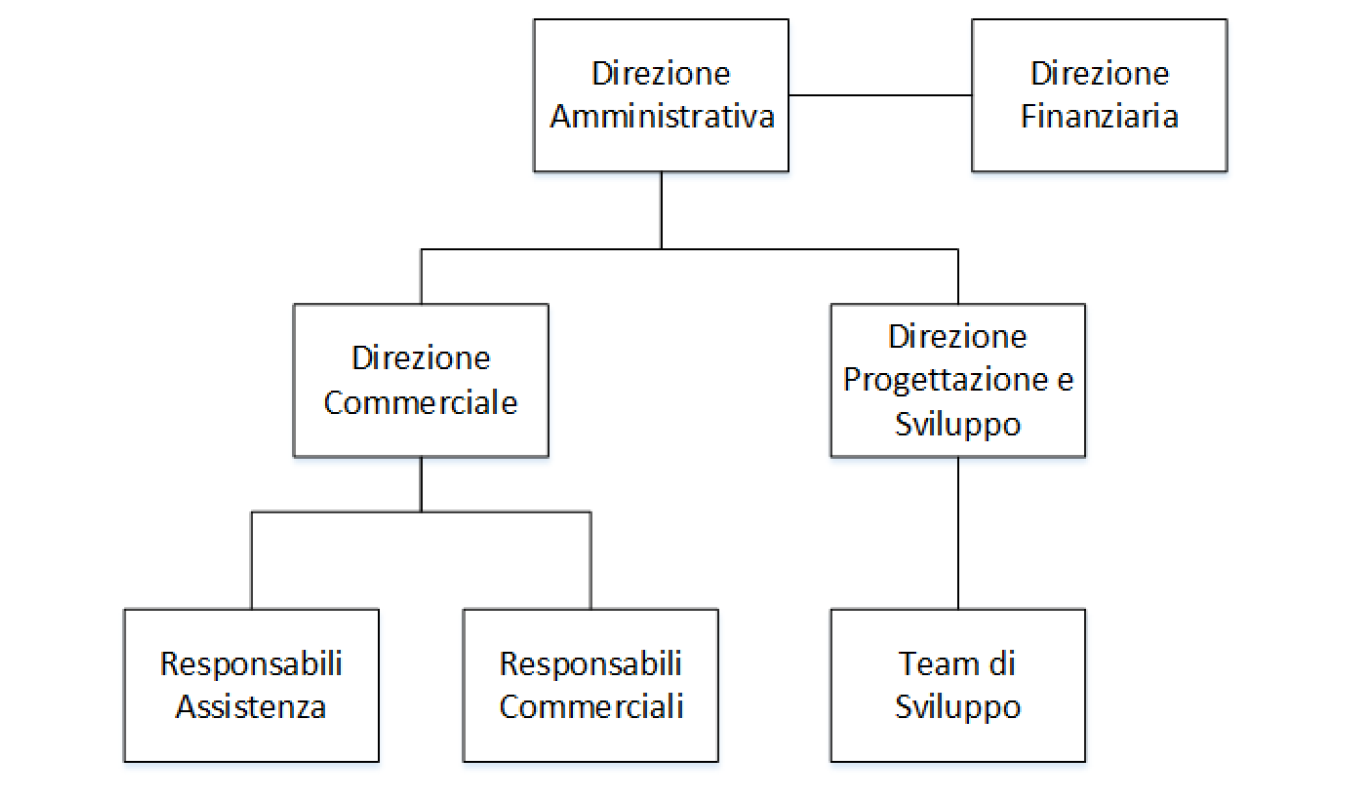
\includegraphics[scale=0.20]{immagini/azienda/struttura_aziendale}
	\caption{\textit{Struttura aziendale \asi}}
\end{figure}\FloatBarrier

Diventa partner IBM dal 1990 e partner Microsoft nel 2000, ASI ha introdotto con largo anticipo, nel 2001, l'utilizzo di servizi cloud nella gestione delle risorse umane, estendendoli in seguito anche ad altri ambiti come i servizi di logistica e di previsione della domanda.

\begin{figure}[ht]
	\centering
	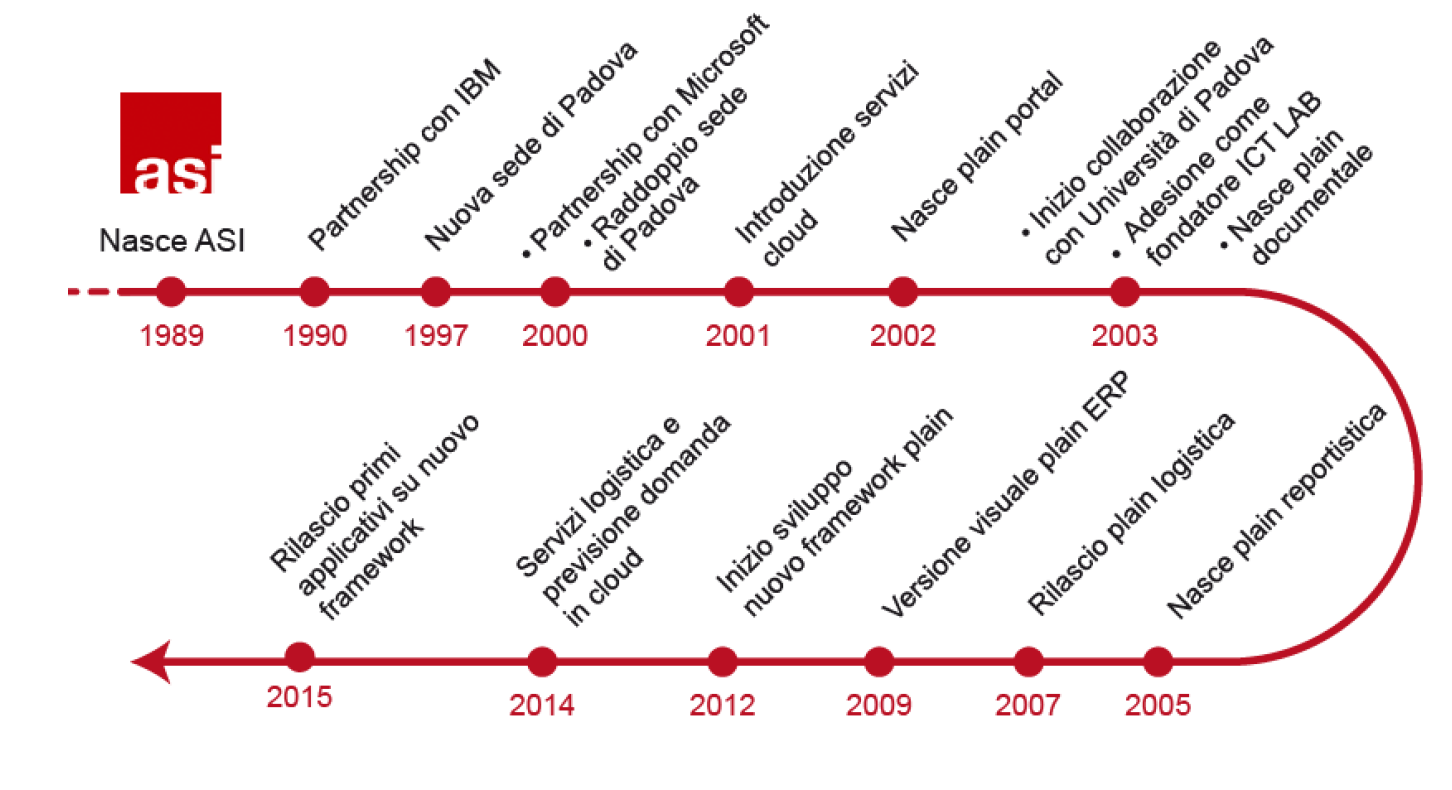
\includegraphics[scale=0.25]{immagini/azienda/timeline}
	\caption{\textit{\textit{Timeline \asi}}}
\end{figure}\FloatBarrier

ASI è associata a Confindustria ed è tra i fondatori di ICTLAB, un gruppo di aziende promosso dalla sezione dei servizi innovativi di Confindustria Padova, allo scopo di contribuire alla sviluppo di un polo produttivo Veneto nel settore delle tecnologie ICT (Information andf Communication Technology, letteralmente " tecnologie dell'informazione e della comunicazione "), inoltre ASI collabora da anni con il Dipartimento di Matematica dell'università di Padova. su progetti di ricerca e sviluppo che interessano la tecnologia ed i prodotti su cui opera.
\\\\
ASI è presente principalmente in Italia settentrionale con circa 200 aziende clienti. Grazie alla flessibilità del prodotto Plain è in grado di servire sia aziende di modeste dimensioni con meno di 50 dipendenti e fatturati sotto i 5 milioni, sia aziende con oltre 500 dipendenti che superano i 50 milioni di fatturato.

\begin{figure}[ht]
	\centering
	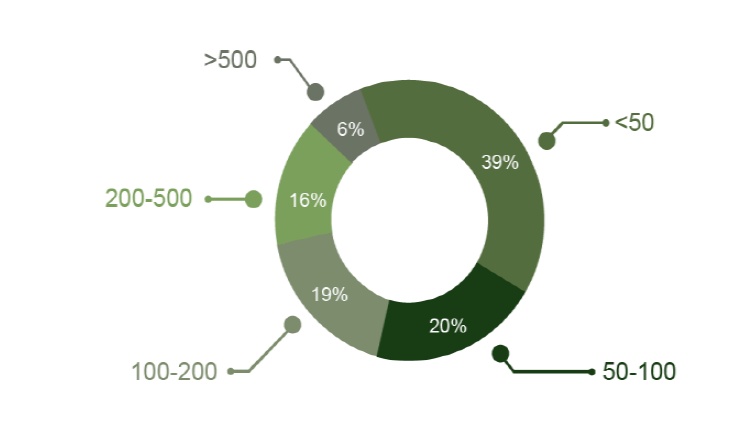
\includegraphics[scale=0.35]{immagini/azienda/dipendenti_clienti}
	\caption{\textit{Dipendenti Clienti \asi}}
\end{figure}\FloatBarrier

\begin{figure}[ht]
	\centering
	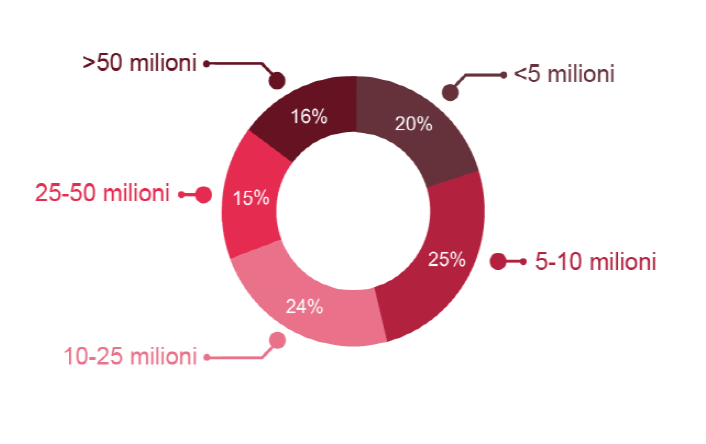
\includegraphics[scale=0.35]{immagini/azienda/fatturato_clienti}
	\caption{\textit{Fatturato Clienti \asi}}
\end{figure}\FloatBarrier

I prodotti e le soluzioni ASI sono pubblicizzati localmente tramite presenza di fiere di settore, tele-marketing mirato utilizzando aziende specializzate, passaparola di clienti soddisfatti.
\\\\
Globalmente vengono invece pubblicizzati attraverso il portale web e con campagne di annunci su Google, tramite \textit{adwords}.
\\\\
Il successo di ASI non deriva solamente dalla qualità del prodotto Plain, ma anche dall'approccio consulenziale  che utilizza con i suoi clienti e dal metodo operativo che applica ad ogni progetto intrapreso.
\section{Processi Aziendali}
\subsection{Processi interni}
Per la gestione dei propri processi aziendali, ASI ha sviluppato un sistema basato sui prodotti Plain, calibrato sulle proprie esigenze, applicando il medesimo approccio che l'azienda utilizza per i suoi clienti.
\\\\
Nel frattempo, ASI sfrutta il proprio sistema anche come ambiente di prova, sperimentando l'efficacia di nuove funzionalità in una situazione di lavoro reale.
\subsubsection{Tecnologie adottate}
Per i processi di sviluppo del proprio software, ASI applica la metodologia Scrum.\\
Si tratta di una metodologia incrementale di sviluppo agile creata da Miocrosoft. la quale suddivide l'intero processo di creazione del software in diverse serie di attività di breve durata (Sprint), che vengono strutturate per perseguire un obiettivo generale definito in precedenza, valutando, al termine di ogni Sprint, gli incrementi ottenuti e la quantità di Sprint ancora necessarie per raggiungere l'obiettivo prestabilito.
\\\\
Tale metodologia consente di monitorare e modificare più facilmente la direzione del progetto, per meglio adattare il prodotto alle richieste del cliente.
\subsection{Processi esterni}
\subsubsection{Approccio consulenziale}
Valutata la tipologia dell'azienda cliente, ASI invia un dipendente commerciale scelto per la sua conoscenza del settore in cui opera il cliente, in modo da assicurare l'utilizzo di un linguaggio largamente condiviso, anche nelle forme gergali cui il cliente è abituato, per favorire la migliore comunicazione possibile ed una analisi più efficace delle esigenze dell'azienda contattata.
\\\\
Durante il primo approccio l'attenzione viene focalizzata non solo sui tempi di realizzazione e sui costi del progetto che si vuole intraprendere, ma anche sulle risorse dell'azienda cliente che possono essere coinvolte, in modo da condividere il più possibile la definizione degli obiettivi del progetto, ponendo il valore aggiunto di ASI sia nell'approfondita competenza tecnica e funzionale, sia nella capacità di stabilire un proficuo rapporto umano con la clientela.
\subsubsection{Startup di progetto}

\begin{figure}[ht]
	\centering
	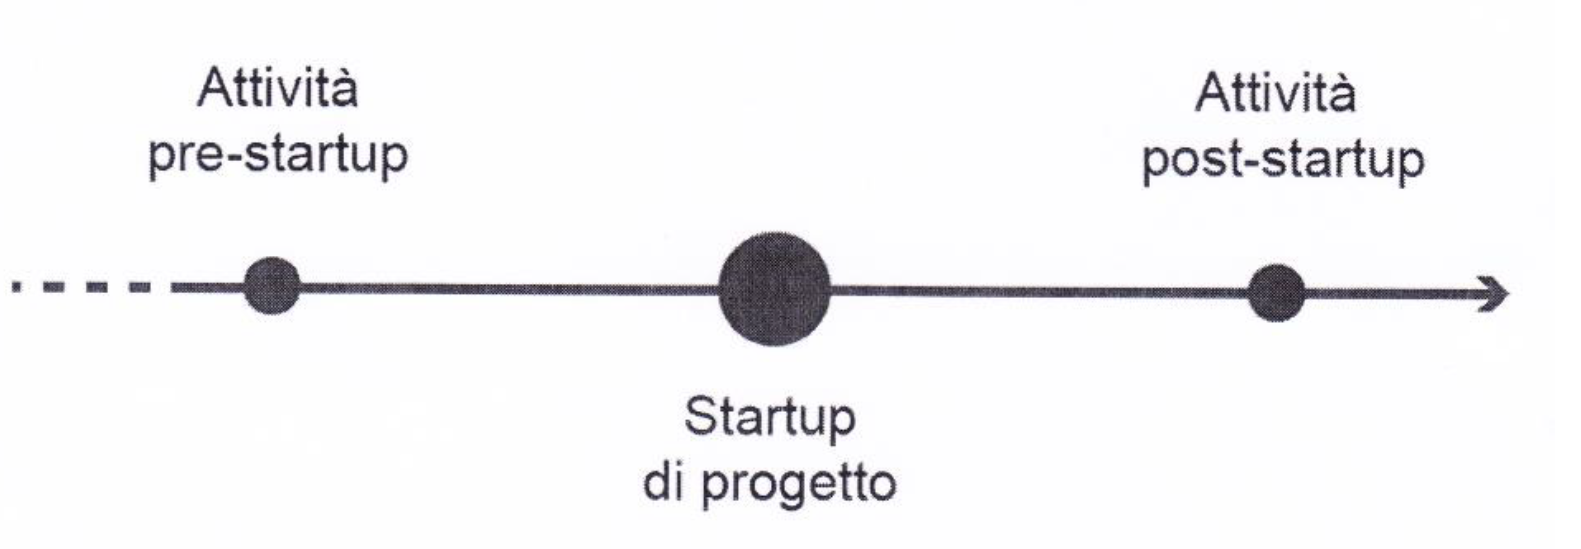
\includegraphics[scale=0.25]{immagini/azienda/startup_di_progetto}
	\caption{\textit{Startup di progetto}}
\end{figure}\FloatBarrier

Una volta confermato l'interessamento del cliente nell'applicazione di uno o più prodotti Plain, inizia lo Startup di progetto, normalmente suddiviso in tre sezioni di attività:
\begin{itemize}
	\item attività Pre-Startup;
	\item attività di Startup;
	\item attività Post-Startup;
\end{itemize}
La metodologia di progetto ASI consente di pianificare gli interventi nel modo più consono alle dimensioni e alle potenzialità dell'azienda cliente, garantendo sempre ed in ogni caso l'accesso alle migliori competenze e alle soluzioni più efficaci, senza mai rinunciare agli standard qqualitativi prefissati.
\paragraph{Attività Pre-Startup}
Le attività Pre-Startup comprendono principalmente l'analisi dell'ambiente e delle necessità del cliente e la progettazione del prodotto, nel pieno rispetto dei bisogni e della struttura dell'azienda.
\\\\
Durante l'approccio consulenziale vengono definite le dimensioni e le possibilità economiche e strutturali dell'azienda, dando una prima definizione della complessità del progetto da intraprendere, adattando di conseguenza lo sforzo delle risorse di ASI.
\\\\
Viene quindi designato un adeguato numero di coordinatori di progetto, a seconda della complessità rilevata; al minimo due: uno di riferimento commerciale per l'azienda cliente, solitamente il dipendente che ha effettuato l'approccio consulenziale, ed uno di riferimento tecnico.
\\\\
In caso di progetto ad alta complessità, possono essere incaricati diversi coordinatori, in modo che ciascuno copra una specifica area tecnica per poter meglio gestire il lavoro; uno di loro assume il ruolo di direttore di progetto per organizzare le varie attività dei coordinatori;
\\\\
Una volta individuate queste figure, grazie alla loro esperienza tecnica viene analizzata in dettaglio la direzione dell'azienda cliente, per ottenere una lista più dettagliata degli obiettivi e delle priorità di quest'ultima, e si prendono in esame eventuali sistemi preesistenti, per favorire una più semplice rivelazione dei fabbisogni informativi ed una migliore definizione della struttura tecnologica da adottare; vengono inoltre individuate le funzioni aziendali coinvolte e le eventuali deleghe necessarie per avviare il progetto.

\paragraph{Attività Startup}
Le attività di Startup comprendono le attività di pianificazione e gestione del lavoro oltre che l'effettiva installazione degli applicativi e la formazione del personale.
\\\\
Sfruttando le analisi effettuate nelle attività di Pre-Startup viene redatto un piano di lavoro che definisce in dettaglio:
\begin{itemize}
	\item le attività da svolgere, aspetti organizzativi del progetto e le relative tempistiche;
	\item i ruoli e le responsabilità delle risorse coinvolte nel progetto, siano esse di ASI o dell'azienda cliente;
	\item l'eventuale conversione di archivi informativi preesistenti in formati fruibili dai prodotti Plain;
	\item la stesura della documentazione di planning del progetto;
	\item la presentazione del progetgto ai partecipanti ed eventuali interessati;
\end{itemize}
Si procede inoltre ad effettuare una mappatura dei processi coinvolti per poter meglio gestire il progredire delle attività in corso, arrivando infine all'installazione dei programmi applicativi, durante la quale viene inizialmente creato un ambiente di prova per testare le piene funzionalità dei prodotti da installare e, solo successivamente, si svolge la parametrizzazione ed installazione del sistema prodotto.
\\\\
Infine avviene la stesura della documentazione di configurazione del sistema e della documentazione sulle scelte di intervento ed i relativi vantaggi attesi.
\\\\
Al termine dell'installazione del sistema vengono avviate attività di sviluppo di eventuali funzionalità addizionali personalizzate per l'azienda cliente.
\\\\
Le ultime attività di Startup comprendono la formazione del personale ed il collaudo in loco del sistema.
\\\\
Sono inoltre previste sessioni specifiche per ciascun utente delle aree coinvolte, in modo che il personale chiave dell'azienda cliente sia perfettamente in grado di utilizzare il prodotto in tutte le sue funzionalità; viene eventualmente fornita a corredo una documentazione specifica per esigenze di maggiore chiarezza sulle procedure operative del sistema e sulle regole aziendali da mantenere.
\\\\
Vengono infine effettuate operazioni di verifica di tutte le funzionalità inserite nel sistema e, solamente dopo aver ottenuto conferma della piena operatività, il sistema viene effettivamente avviato all'interno dell'azienda cliente.

\paragraph{Attività Post-Startup}
Le attività di Post-Startup comprendono le attività di ulteriore personalizzazione e perfezionamento del sistema informatico installato, assicurando che le funzionalità del prodotto corrispondano esattamente alle esigenze del cliente.
\\\\
Viene inoltre offerto un piano di supporto calibrato sulle possibilità dell'azienda, iniziando da soluzioni più standardizzate arrivando ad una serie di strumenti elaborati ad hoc, mantenendo in ogni caso un affiancamento tecnico agli utenti aziendali per garantire la massima tranquillità operativa di questi ultimi.
\\\\
Si concorda infine con il cliente un piano di mantenimento e di verifica del sistema, la cui durata può variare da uno a diciotto mesi, secondo la complessità definita precedentemente.

\section{Plain}
Plain è una suite di soluzioni software sviluppata da \asi per supportare principalmente la gestione delle aziende che hanno specifiche competenze in ambiti produttivi e commerciali; tutti i prodotti forniti condividono una serie di caratteristiche e funzionalità che li accomunano e che ne qualificano la metodologia di sviluppo.

\subsection{Caratteristiche}
Le soluzioni Plain sono caratterizzate da un'architettura scalabile ed aperta all'utilizzo in rete, in grado di gestire efficacemente un qualsiasi volume di utenti o dati, anche su cloud, per permettere la fruibilità ad aziende di qualsiasi dimensione; forniscono inoltre un'ampia configurabilità per permettere:
\begin{itemize}
	\item una profonda adattabilità al contesto organizzativo in cui vengono inserite, in modo da adattarsi sia alla tipologia dell'azienda, sia agli eventuali sistemi informatici già utilizzati, modificando il meno possibile le abitudini dei clienti;
	\item un'alta navigabilità, puntando ad ottenere tutte le informazioni disponibili, collegate ad un soggetto (un cliente, un fornitore, un articolo o altro), il più efficacemente possibile;
	\item una gestione puntuale della sicurezza e riservatezza nell'accesso ai dati, sia all'interno, che all'esterno dell'azienda;
\end{itemize}
Le soluzioni Plain inoltre contengono una serie di funzionalità condivise:
\begin{itemize}
	\item la personalizzazione delle interfacce utente, come i cruscotti aziendali, le KPI (Key Performance Indicatrors o indicatori chiave di prestazioni), le relazioni tra documenti e la navigabilità, che consente di aver un sistema a supporto dell'utente e non il contrario;
	\item gestione documentale, reportistica (analisi e statistiche) e KPI integrate nella soluzione gestionale e disponibili in ogni momento per restituire informazioni contestualizzate;
	\item modulo BPM (Business Process Management) integrato per la modellazione dei flussi di lavoro;
	\item connettori con soluzioni specialistiche dipartimentali, come la tesoreria, CRM (Customer Relationship Management o gestione delle relazioni con i clienti), e-commerce etc.;
	\item base di dati accessibile da qualsiasi piattaforma con strumenti di analisi o Business Intelligence;
\end{itemize}
\subsubsection{Soluzioni Plain principali}
\begin{itemize}
	\item \textbf{Plain ERP industria}, si tratta di una piattaforma creata per fornire supporto a tutte le attività gestionali di un'azienda di produzione industriale, raccogliendo i moduli applicativi in 8 aree funzionali (amministrazione, finanziaria, di controllo, vendite, approvvigionamenti, magazzino, produzione ed integrazione), con specializzazione negli ambiti della produzione metalmeccanica, sia in serie che su commessa, e sullo stampaggio ed estrusione di materie plastiche.
	
	\begin{figure}[ht]
		\centering
		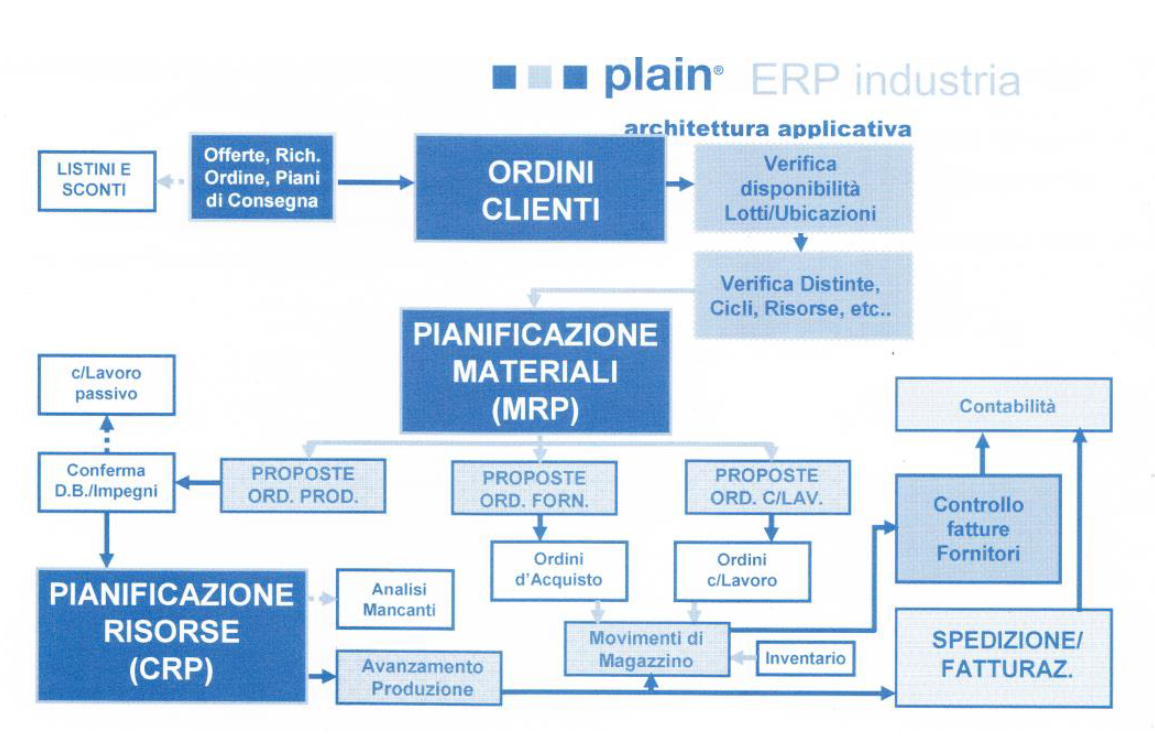
\includegraphics[scale=0.40]{immagini/azienda/plain_erp_industria}
		\caption{\textit{Plain ERP Industria}}
	\end{figure}\FloatBarrier
	
	\item \textbf{Plain ERP Commercio}, soluzione specificatamente destinata alle attività gestionali di un'azienda commerciale, i cui moduli applicativi sono raccolti in 9 aree funzionali (amministrazione, finanziaria, di controllo, vendite, approvvigionamenti, magazzino, assistenza tecnica, lavorazioni ed integrazione), con specializzazione nei mercati della carta e cancelleria (grossisti, fornituristi e cash), giocattoli ed articoli da regalo, ricambi (sia automotive che industriali), nonché ferramenta ed utensileria.
	
	\begin{figure}[ht]
		\centering
		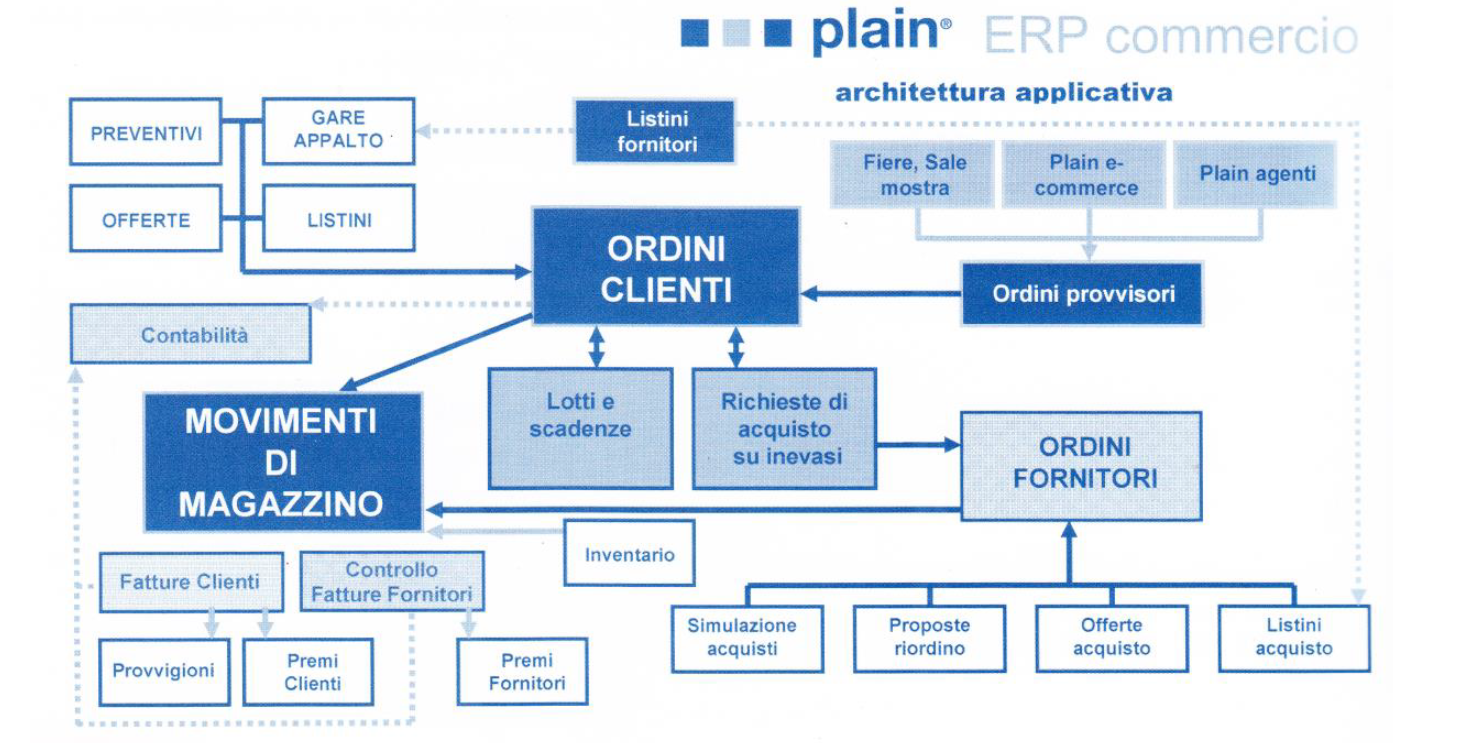
\includegraphics[scale=0.35]{immagini/azienda/plain_erp_commercio}
		\caption{\textit{Plain ERP Commercio}}
	\end{figure}\FloatBarrier
	
\end{itemize}
\subsubsection{Altre soluzioni Plain}
Plain fornisce ulteriori soluzioni applicabili in qualsiasi ambito aziendale oppure destinate a specifiche tipologie di azienda; queste soluzioni possono essere di supporto anche ai due principali ERP Plain, applicabili singolarmente o interfacciate con ERP già esistenti:
\begin{itemize}
	\item Plain Logistica, studiata principalmente per grossisti di carta e cancellerie o fornituristi di ufficio, fornisce un sistema per la migliore gestione dei magazzini e dei processo di movimento della merce;
	\item Plain Previsione Domanda, studiata principalmente per grossisti di carta e cancellerie o fornituristi di ufficio, fornisce un sistema per tracciare ed analizzare le vendite ed acquisti, per rendere più efficace ed efficiente gestire le richieste dei clienti;
	\item Plain Documentale, applicabile in qualsiasi ambito aziendale, fornisce un sistema efficiente per archiviare, gestire, accedere e condividere i documenti aziendali;
	\item Plain HR (human resource), applicabile in qualsiasi ambito aziendale, fornisce un sistema per gestire tutti gli aspetti riguardanti le risorse umane in azienda;
	\item Plain Extended data publisher, applicabile in qualsiasi ambito aziendale, fornisce un sistema per gestire ed ottenere facilmente ed efficacemente le informazioni contenute nei sistemi informativi aziendali in qualsiasi momento;
	\item Plain Presenze, applicabile in qualsiasi ambito aziendale, fornisce un sistema per la rilevazione delle presenze interfacciabile con qualsiasi sistema di rilevamento delle timbrature, automatizzando i controlli periodici sulle risorse;
\end{itemize}
\subsection{Propensione all'innovazione}
ASI punta principalmente a mantenere efficace e competitiva la propria suite di prodotti Plain, sfruttando la sua adattabilità per adeguarsi alla tecnologia utilizzata nelle aziende clienti.
\\\\
L'azienda monitora costantemente le nuove tecnologie rilasciate sul mercato, cercando di individuare quelle che possano essere assimilate in tutto o in parte nella propria suite di prodotti, o che possano costituire la base per lo sviluppo di un nuovo prodotto Plain.
\\\\
Grazie al suo crescente successo, ASI è stata in grado di investire una sempre maggiore percentuale del suo fatturato nella ricerca e sviluppo dei prodotti Plain, raggiungendo circa il 22\% nel 2015; mantenendo così la suite Plain in costante evoluzione, grazie ad almeno tre aggiornamenti all'anno.
\\\\
Per valutare l'efficacia e l'eventuale utilizzo di nuove tecnologie, ASI svolge innanzitutto una prima analisi per individuare in dettaglio le funzionalità e caratteristiche che possono portare migliorie o aggiunte all'interno dei prodotti Plain, cercando di definire i costi e la quantità di lavoro necessaria per la loro implementazione.
\\
Se l'analisi effettuata porta risultati soddisfacenti vengono allestiti progetti per sviluppare implementazioni di prova, i quali possono essere portati a termine interamente da membri del team di sviluppo, ma che spesso vengono proposto come esperienze di stage tramite l'Università di Padova.

             % Introduzione
\newpage
%**************************************************************
\chapter{Lo Stage}
%********

\section{Utilizzo degli stage in azienda}
Tramite la convenzione con l'Università di Padova, ASI propone, da circa un decennio, progetti di stage orientati allo sviluppo di integrazioni per i suoi prodotti della suite Plain, basati principalmente sulle più recenti tecnologie.
\\
Le tecnologie e le eventuali integrazioni vengono preventivamente analizzate dal team di sviluppo, per assicurare un apporto di valore ai prodotti Plain interessati e per meglio definire gli obiettivi attesi dai progetti di stage.
\\
Dai progetti di stage ASI si ripromette di ottenere non solo un prototipo funzionante, potenzialmente integrabile nella propria suite, ma anche una valutazione più approfondita della tecnologia utilizzata, in modo da determinare l'effettivo valore aggiunto, i costi della sua implementazione, sia in termini di tempo sia di risorse, e l'eventuale interesse aziendale nel completamento dello sviluppo del prototipo e nell'utilizzo di tale tecnologia in prodotti futuri.
\\
Tramite i progetti di stage ASI ha inoltre la possibilità di valutare l'operato degli stagisti, sia sul piano professionale che comportamentale, proponendo eventualmente di portare a termine il prodotto sviluppato durante lo stage o valutando altre forme di collaborazione, anche in vista di una possibile assunzione.

\section{Collocazione degli stagisti}
Dopo un colloquio preliminare, in cui ciascuna delle parti manifesta il reciproco interesse nel progetto proposto, lo stagista viene inserito direttamente nel team di sviluppo di ASI, dove gli vengono inizialmente spiegate le metodologie utilizzate e gli standard aziendali da osservare nella scrittura del codice e nella redazione di eventuali documenti.

\section{Metodologia di sviluppo: Scrum}
Come metodologia di sviluppo, ASI adotta \textbf{Scrum}, un framework\ped{G} agile\ped{G} per lo sviluppo del software.
\\\\
\textit{"Scrum è un framework di processo utilizzato dai primi anni '90 per gestire lo sviluppo di prodotti complessi. Scrum non è un processo o una tecnica per costruire prodotti, ma piuttosto è un framework all'interno del quale è possibile utilizzare vari processi e tecniche. Scrum rende chiara l'efficacia relativa del tuo product management e delle prtiche di sviluppo usate in modo da poterle migliorare." (Jeff Sutherland "La Guida a Scrum")}
\begin{figure}[ht]
	\centering
	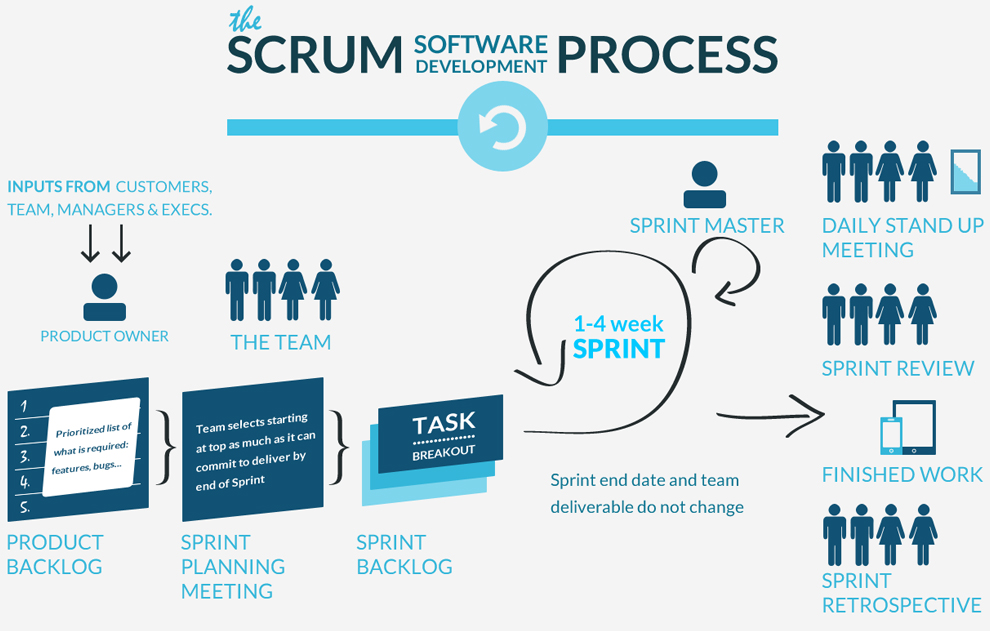
\includegraphics[scale=0.35]{immagini/processo/Scrum.jpg}
	\caption{\textit{Processo di sviluppo Scrum}}
\end{figure}\FloatBarrier

\subsection{Il processo Scrum}
Il processo Scrum è stato ideato da Jeff Sutherland e Ken Schwaber nei primi anni '90, i quali lo hanno codificato e presentato nel 1995 alla conferenza OOPSLA\ped{G} (Object-Oriented Programming, System, Languages \& Applications), pubblicando "Scrum Sofware Development Process".
\\
Il nome 'Scrum', un termine riferito alla mischia nel rugby, è stato preso da un testo del 1986, \textit{'The New Product Development Game'}, scritto da Ikujiro Nonaka e Hirotaka Takeuchi, nel quale venne introdotta una prima idea dello Scrum di oggi.
\\
Nel loro testo vengono appunto evidenziate numerose analogie tra le squadre nel gioco del rugby ed i team di sviluppo nella produzione di software, spiegando come le migliori prestazioni nello sviluppo di prodotti complessi si ottengono quando ai team, considerati come piccole, indipendenti unità di persone, vengono assegnati obiettivi piuttosto che attività, dimostrando che i team migliori sono quelli che hanno la possibilità di studiare le proprie tattiche su come arrivare all'obiettivo condiviso.

\subsection{La teoria Scrum}
La teoria di Scrum si basa sul processo di controllo empirico, il quale afferma che la conoscenza scaturisce dall'esperienza e nel prendere decisioni basate su ciò che si sia, applicando quindi un approccio incrementale e iterativo per ottimizzare la prevedibilità e controllare i rischi, sfruttando tre pilastri di base:
\begin{enumerate}
	\item Trasparenza \\ Gli aspetti rilevanti del processo devono essere visibili ai responsabili del risultato dello stesso, inoltre tali aspetti devono essere definiti da uno standard comune per consentire agli osservatori di comprendere quello che vedono, per esempio un linguaggio comune per riferirsi al processo e una definizione comune per il termine del processo.
	\item Ispezione \\ Gli utilizzatori di Scrum devono frequentemente analizzare gli artefatti prodotti ed i progressi ottenuti per il conseguimento degli obiettivi preposti, per identificare variazioni inaspettate. Tali verifiche non devono essere troppo frequenti e sono più utili se effettuate da appositi ispettori nel posto di lavoro.
	\item Adattamento \\ Se un ispettore determina che uno o più aspetti di un processo deviano dai limiti accettabili, deve essere eseguito quanto prima un aggiustamento, per minimizzare future deviazioni.
\end{enumerate}

\subsection{Ruoli Scrum}
\subsubsection{Product Owner}
Il product Owner rappresenta gli stakeholder\ped{G} ed ha il ruolo di massimizzare il valore del prodotto del Team di Sviluppo, definendo i requisiti del prodotto e la loro priorità, aggiungendoli al Product Backlog. Il product Owner è necessario per un team Scrum e si raccomanda che non sia combinato con il ruolo di Scrum Master.
\subsubsection{Scrum Master}
Lo Scrum Master fa in modo che Scrum sia compreso e messo in atto, assicurandosi che il Team di Sviluppo aderisca alla teoria, alle pratiche e alle regole Scrum, facendo in modo che, anche gli operatori esterni al team Scrum, capiscano quali iterazioni aiutino il team e quali siano dannose, massimizzando il valore creato dal team.
\subsubsection{Team di Sviluppo}
Il Team di Sviluppo consiste in un piccolo numero di professionisti che si occupano di creare gli incrementi che portano al raggiungimento dell'obiettivo della Sprint.
\\
La dimensione di un Team di Sviluppo solitamente è fra tre e i nove membri; poiché averne meno di tre riduce di troppo l'iterazione tra i membri ed averne più di nove aumenta eccessivamente la complessità di gestione.
\subsubsection{Artefatti Scrum}
Gli Artefatti Scrum rappresentano metodi per ottenere trasparenza ed opportunità di ispezione e adattamento, creati per massimizzare la trasparenza dei valori chiave, facendo in modo che tutti abbiano ua piena conoscenza dell'artefatto.
\subsubsection{Product Backlog}
Il Product Backlog è una lista ordinata di tutto ciò che può essere utile riguardo al prodotto e viene utilizzato come unica fonte di requisiti per qualsiasi cambiamento da apportare; il Product Owner è responsabile di mantenere aggiornato il Product Backlog in tutti i suoi aspetti, sia nel contenuto che nell'ordinamento.
\\
Il Product Backlog non è mai completo, in quanto comprende una lista che evolve dinamicamente con lo sviluppo del prodotto, identificando quali sono le caratteristiche che il prodotto deve avere per essere appropriato, utile e competitivo.
\\
Nel Product Backlog sono riportate tutte le funzionalità, i requisiti, i miglioramenti e le correzioni che costituiscono tutti i cambiamenti che devono essere effettuati al prodotto in rilasci futuri, gli oggetti nel Product Backlog sono tutti dotati di una descrizione, una priorità ed un valore che ne definisce lo sforzo previsto per apportare la modifica.
\\
Oggetti con priorità più alta sono solitamente meglio descritti che quelli con priorità bassa, per aiutare il Team di Sviluppo a concentrarsi sui cambiamenti più impellenti.
\subsection{La Sprint}
Il cuore di Scrum sono le Sprint: si tratta di un'unità di tempo, la cui durata può variare da una settimana ad un mese, durante la quale viene creato un incremento di prodotto utilizzabile e potenzialmente rilasciabile. In ciascuna Sprint si definisce lo scopo da raggiungere ed un piano che aiuti nello sviluppo, viene realizzato il lavoro di sviluppo ed il prodotto risultante.
\\
Le Sprint possono essere cancellate unicamente dal Product Owner, solitamente quando non ha più senso proseguire a causa di mutamenti di direzione dell'azienda, del mercato o delle tecnologie che ne rendano obsoleto l'obiettivo.
\\
Le attività che definiscono il lavoro di una Sprint consistono in:
\begin{itemize}
	\item \textbf{Pianificazione della Sprint} \\
	Nella fase di Pianificazione della Sprint tutto il team Scrum collabora per definire l'obiettivo generale basandosi principalmente sul Product Backlog, sull'ultimo incremento del prodotto, sulla previsione della capacità del Team di Sviluppo sulle loro prestazioni passate, aiutando a specificare cosa può essere fatto durante la Sprint e le modalità per ottenere l'incremento desiderato.
	\item \textbf{Scrum Giornalieri} \\
	Gli Scrum Giornalieri sono dei brevi incontri, di circa quindici minuti, del Team di Sviluppo per sincronizzare le proprie attività; ogni membro del team spiega cosa ha realizzato nel giorno precedente, cosa considera di fare nel giorno corrente e se ha riscontrato difficoltà impreviste che possono impedire o rallentare il raggiungimento dell'obiettivo predefinito. Gli Scrum Giornalieri sono utilizzati per valutare i progressi verso l'obiettivo della Sprint di volta in volta e per definire efficacemente le prestazioni del Team di Sviluppo.
	\item \textbf{Revisione Sprint} \\
	Nella revisione della Sprint si analizza l'incremento ottenuto e si aggiorna il Product Backlog, se necessario, collaborando con gli stakeholders per definire come ottimizzare il valore degli incrementi.
	\\
	La Revisione Sprint è un incontro informale e la presentazione dell'incremento punta a sollecitare i feedback e ad aumentare la collaborazione tra le parti.
	\\
	Solitamente una Revisione Sprint dura quattro ore per Sprint di un mese, mentre può durare meno in casi di Sprint più brevi, a discrezione dello Scrum Master.
	\item \textbf{Retrospettiva Sprint} \\
	La Retrospettiva Sprint avviene subito dopo la Revisione e prima della nuova Pianificazione ed è utilizzata dal team Scrum per ispezionare il proprio lavoro, individuando come sono progredite le attività assegnate, identificare quali sono state le problematiche più importanti e pianificare metodi per migliorare le modalità di lavoro del team.
	\\
	LA Retrospettiva Sprint dura al massimo tre ore, secondo la durata della Sprint
\end{itemize}

Nei suoi processi di sviluppo software ASi adotta la metodologia Scrum, che fornisce strumenti particolarmente adeguati alle proprie modalità di rapportarsi con i clienti, garantendo affidabilità nelle tempistiche e nelle personalizzazioni, nonché le opportune interazioni con gli stakeholders.
\\
La suddivisione del lavoro in Sprint definisce, infatti, con buona precisione, i tempi di sviluppo e consente, grazie alla breve durata di ogni Sprint, di migliorare l'andamento del lavoro per meglio confrontarsi alle richieste del cliente.
\\
Le revisioni previste da ogni Sprint impongono inoltre un confronto diretto con i committenti, favorendo la definizione delle loro esigenze e precisando i requisiti da soddisfare nelle Sprint future.
\\
La metodologia Scrum, che prevede di ottenere sempre un incremento funzionale al termine di ogni Sprint, favorisce pertanto l'applicazione di correzioni o integrazioni puntuali a progetti già avviati, ottenendo il progressivo affinamento dei prodotti della suite Plain, sia per quelli in fase di sviluppo, sia per quelli già rilasciati.

\subsection{Tecnologie usate dall'azienda}
\subsubsection{.NET}

\begin{figure}[ht]
	\centering
	
\includegraphics[scale=0.40]{immagini/processo/DotNet.jpg}
	\caption{\textit{Funzionalità versioni .NET}}
\end{figure}\FloatBarrier

ASI, essendo una consolidata partner Microsoft, sfrutta come base per lo sviluppo dei suoi progetti la tecnologia .NET di Microsoft, la quale è una piattaforma di sviluppo software indicata per la programmazione ad oggetti, sviluppata da Microsoft come contrapposizione al linguaggio Java.
\\
Diffusa la prima volta nel 2002, .NET ottenne subito un vantaggio su Java diventando standard ISO nel 2003 (ISO 23270 ed ISO 23271) ed avendo come caratteristica di essere indipendente dalla versione di Windows su cui è installata.
\\
.NET è un'implementazione della CLI (Common Language Infrastructure), una specifica che definisce un ambiente che permette a più linguaggi di alto livello di essere utilizzati su differenti piattaforme senza la necessità di essere riscritto.
\\
.NET infatti contiene compilatori per svariati linguaggi forniti da Microsoft (C\#, Visual Basic .NET, JAvaScript, J\#, etc.) e consente di utilizzare altri linguaggi tramite compilatori forniti da produttori di terzi, che traducano il linguaggio di alto livello scelto in CIL (Common Intermediate Language), il linguaggio di livello più basso previsto dalla piattaforma .NET e della CLI, che svolge lo stesso ruolo del Bytecode in Java.
\\
Il CIL è un linguaggio assembly orientato agli oggetti completamente basato su stack.

\begin{figure}[ht]
	\centering
	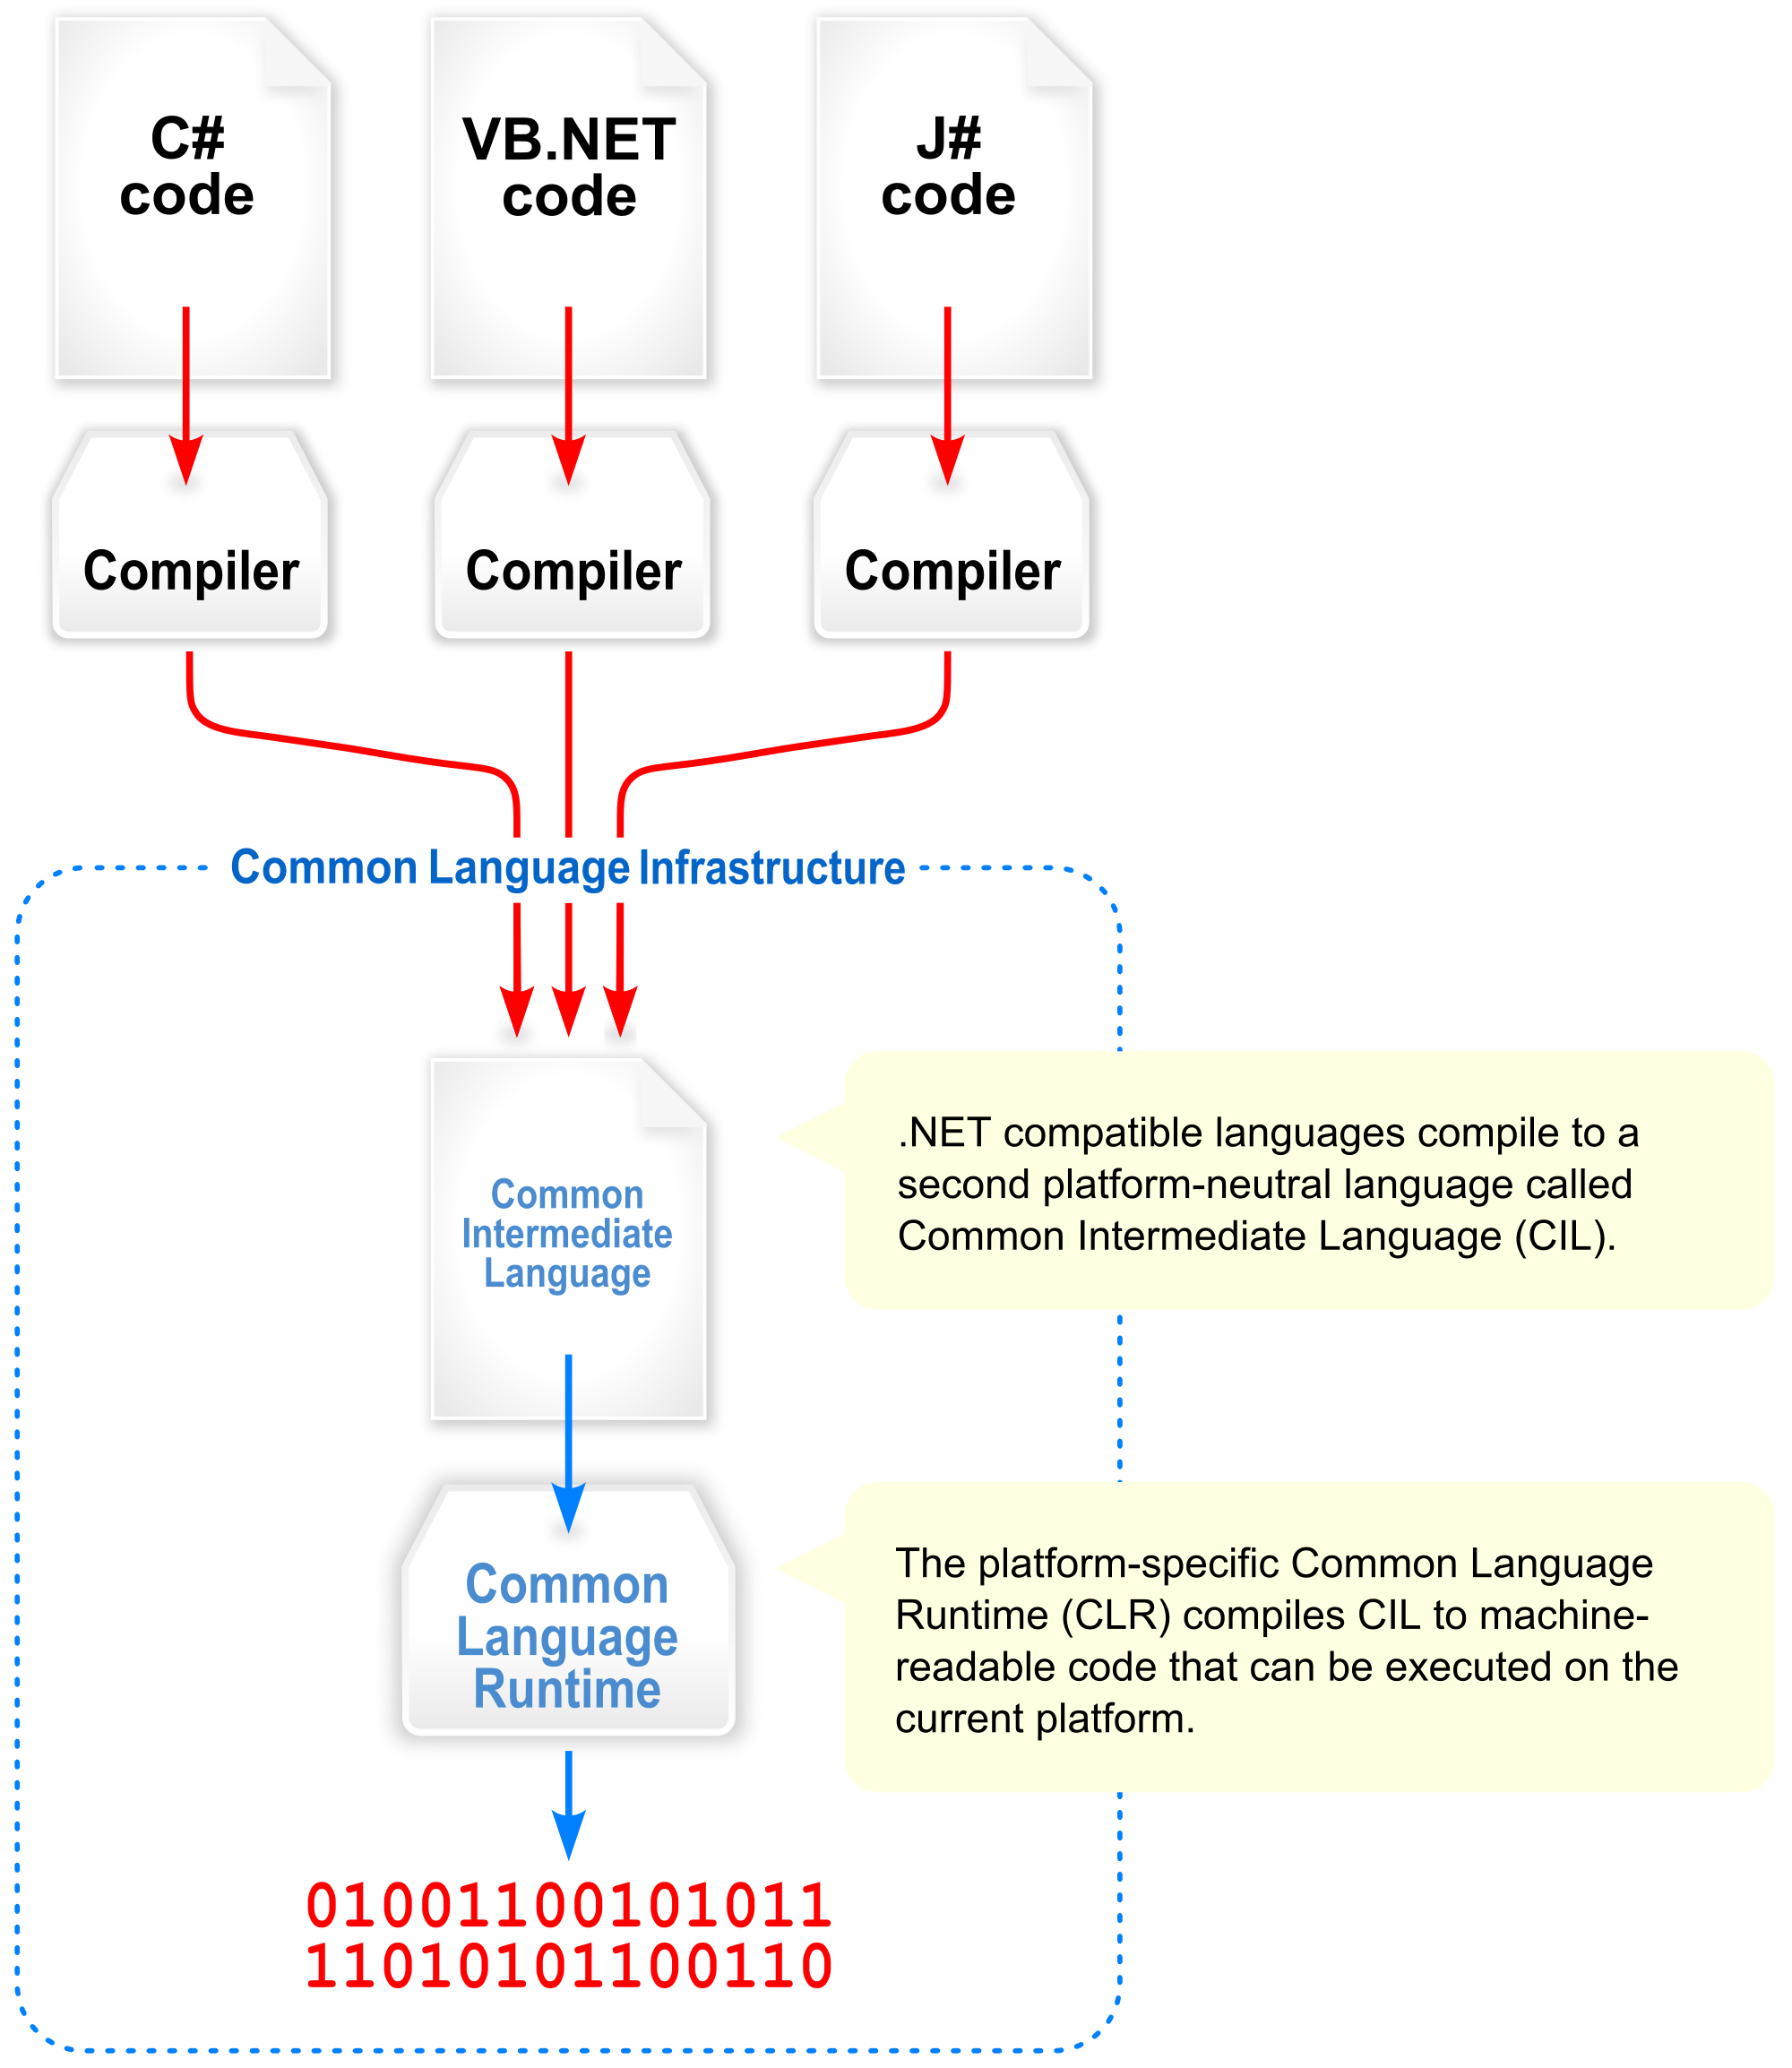
\includegraphics[scale=0.12]{immagini/processo/CIL.png}
	\caption{\textit{Schema Common Language Infrastructure}}
\end{figure}\FloatBarrier

il CLI viene eseguito a Runtime\ped{G} dalla CLR (Common Language Runtime), che rappresenta sia la macchina virtuale di Microsoft, sia le librerie standard della piattaforma .NET.
\\
All'interno dell CLR è presente il CLS (Common Language Specification), un ambiente di esecuzione usato principalmente sui sistemi operativi Microsoft, che i compilatori devono supportare per permettere l'interoperabilità tra i diversi linguaggi di programmazione.
\\
Esistono anche implementazioni per sistemi Unix\ped{G} e Linux\ped{G}, la più famosa denominata Mono è un'implementazione multi-piattaforma del CLS.

\subsubsection{Visual Studio}
Visual Studio è un IDE\ped{G} (Integrated Development Environment) sviluppato da Microsoft per aiutare lo sviluppo di programmi che utilizzano .NET, supportando diversi tipi di linguaggio (C,C++,C\#,F\#,Visual Basic .NET, etc), contenendo un compilatore .NET per tutti i linguaggi supportati, traducendoli in IL (Intermediate Language).
\\
Visual Studio eredita dal suo predecessore, Visual Basic, la tecnologia IntelliSense, che permette di correggere errori sintattici e alcuni logici senza effettuare una compilazione, facilitando la scrittura del codice. Possiede anche un debugger interno per il rilevamento e correzione di errori logici a runtime e fornisce doversi strumenti per l'analisi prestazionale.
\\
Una delle caratteristiche che ha portato ASI ad utilizzare Visual Studio, oltre ad essere l'IDE predefinito per lo sviluppo .NET, è la sua integrazione nativa con l'ambiente di sviluppo di gruppo Team Fondation Server.

\subsubsection{Team Fondation Server}
Team Fondation Server (p TFS) è un set di strumenti per incrementare la collaborazione tra sviluppatori indipendentemente dal linguaggio utilizzato. Tali strumenti interagiscono con l'IDE scelto e sono integrati automaticamente in Visual Studio, aiutando con il controllo della versione, fornendo repository\ped{G} privati per gestire il codice senza dover uscire dall'IDE, con l'integrazione continua, consentendo di compilare e testare la qualità delle applicazioni prodotte dopo ogni modifica, aiutando la distribuzione automatica dei prodotti che superano i test.
\\
Le funzionalità di TFS più utilizzate da ASI forniscono strumenti con Visual Studio per l'implementazione della metodologia Scrum nello sviluppo del prodotto, fornendo svariati strumenti per definire in un modo semplice ed intuitivo il lavoro da svolgere.
\\
TFS fornisce innanzitutto una visualizzazione del Product Backlog per il progetto, dove è possibile visualizzare, inserire e modificare in modo intuitivo gli oggetti nel Product Backlog, ai quali è possibile definire un ampio numero di specifiche, semplificando di molto la creazione e gestione di questo importante artefatto della metodologia Scrum.
\\
TFS consente di pianificare le Sprint da effettuare semplicemente definendo le date di inizio e fine delle stesse, rendendo chiaro il numero di incrementi da apportare e le tempistiche da eseguire. Alle Sprint è poi possibile inserire oggetti del Product Backlog, per precisare gli incrementi che si svolgeranno in quel tempo e per definire la quantità di sforzo necessaria per portare a termine la sprint.
\\
E'possibile inoltre definire i profili utente del Team di Sviluppo, inserendo la quantità di sforzo giornaliero che possono impiegare durante li sprint, il ruolo che ricoprono ed i loro giorno lavorativi, in modo da ottenere in modo semplice la quantità di sforzo applicabile dal Team di Sviluppo nella Sprint che si va a definire. Dopo aver inserito gli oggetti del Product Backlog nella Sprint è possibile collegarli direttamente ai membri del Team di Sviluppo interessati, ottenendo un immediato schema dello sforzo richiesto da ogni membro del Team, consentendo poi di redistribuire gli oggetti in modo che lo sforzo di ogni membro sia utilizzato al massimo dell'efficacia.
\\
Il TFS aiuta a rendere chiaro e intuitivo lo svolgimento del lavoro da parte del Team di Sviluppo a tutti i ruoli interessati ed aiuta i nuovi utenti ad implementare facilmente la metodologia Scrum nel loro progetto.

\section{Scrum in ASI}
Il Team di Sviluppo ASI non ha personalizzato l'approccio a Scrum in alcun modo, il ruolo di Product Owner è stato dato ad uno dei membri fondatori dell'azienda, il quale ha creato il Product Backlog per ogni progetto in corso, gli oggetti al suo interno sono stati definiti 'Task' ed hanno utilizzato la definizione che TFS fornisce per determinare il termine.
\\
Per la gestione delle richieste al Team di Sviluppo da parte degli altri dipendenti dell'azienda, lo Scrum Master ha imposto che venissero inviate tramite inserimento di Task nel relativo progetto a cui la richiesta fa capo, lasciando che fosse il Product Owner poi ad impostarne la priorità per meglio guidare il lavoro degli sviluppatori.
\\
Le Sprint in ASI sono sempre della durata settimanale (10 giorni lavorativi), effettuando solitamente la fase di Revisione e Retrospettiva il lunedì e la fase di Pianificazione della Sprint successiva il martedì.

\section{Obiettivi dello Stage}
L'obiettivo dello stage era la creazione di un applicativo mobile, multi-piattaforma, che permetta la generazione di rapportini firmabili, tramite firma biometrica, in formato pdf.
\\
Mi è stato richiesto inoltre di sviluppare dei servizi che espongono i dati necessari all'applicazione e di realizzare una sincronizzazione intelligente dei dati, dove ciò che transita è solo ciò che effettivamente è stato modificato. 
\\
Per la realizzazione dell'applicazione cross-platform mi è stato richiesto l'uso del framework \textbf{Xamarin.Forms}, un framework per lo sviluppo multi-piattaforma che fornisce varie API per l'applicazione della CLI negli applicativi mobili sfruttando il framework .NET, e consente sopratutto di sviluppare UI\ped{G} (User Interfaces) che possono essere condivise tra dispositivi Android, iOS e Windows Phone, traducendo a runtime il codice condiviso in codice nativo.

\begin{figure}[ht]
	\centering
	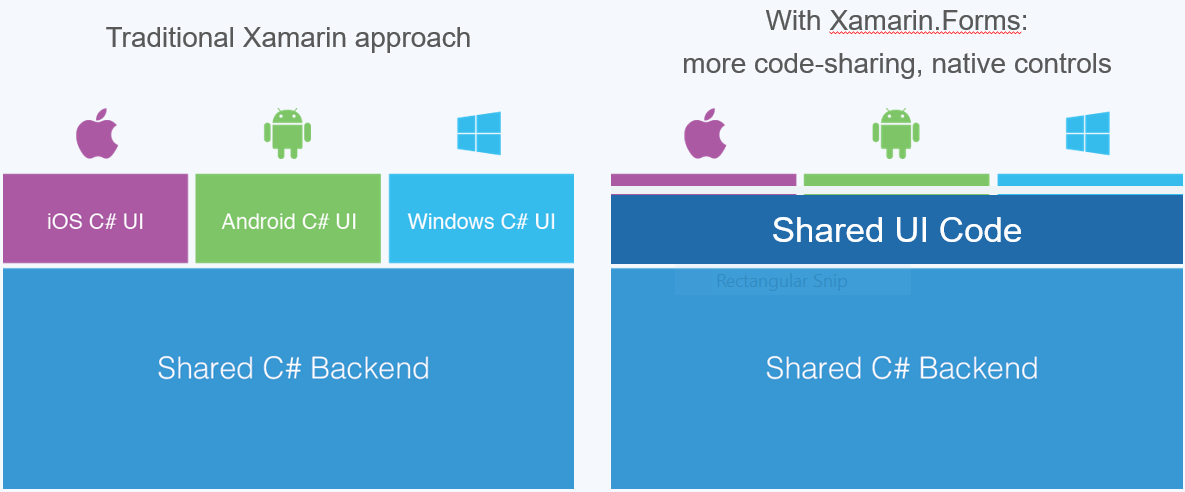
\includegraphics[scale=0.57]{immagini/processo/xamarinForms.png}
	\caption{\textit{Differenza di approccio tra Xamarin e Xamarin.Forms}}
\end{figure}\FloatBarrier

Mi è stato richiesto anche di valutare alcuni modi per gestire la realizzazione di un pdf esclusivamente nel dispositivo mobile a partire da un template\ped{G}, senza creare il documento direttamente via codice. Questa scelta è stata accordata per garantire una elevata manutenibilità del software, che in caso di variazioni del rapportino da emettere, rende semplice la modifica del template.
\\
Sono state valutate varie librerie commerciali per la generazione del pdf a partire da un template, ma nessuna offriva realmente ciò che interessava all'azienda, pertanto si è deciso di puntare in un template XSLT che a partire da un XML con associato un foglio di stile, permette la generazione di una pagina HTML che a sua volta sarà convertita in pdf grazie alle funzionalità offerte da pacchetto iTextSharp.

\subsection{Vincoli del progetto di stage}
Una volta inserito come membro del Team di sviluppo di ASI, mi è stato chiesto di seguire le direttive di sviluppo dei software aziendali, che si ricollegano alle norme di scrittura del codice definite da Microsoft per lo sviluppo .NET.

\subsection{Impostazione del lavoro}
Il lavoro da svolgere durante lo stage è suddiviso in \textbf{fasi},che sono state introdotte in varie Task dal tutor aziendale ed assegnate di volta in volta al mio profilo dallo Scrum Master del Team di sviluppo, alla Pianificazione di ogni Sprint.
\begin{itemize}
	\item[I.] La prima fase è stata dedicata alle conoscenze generali per approfondire le conoscenze del .NET Framework 4.5 e familiarizzare con gli strumenti integrati in Visual Studio, quali TFS, Testing e Continuous integration.
	\item[II.] La seconda fase è stata dedicata all'acquisizione degli standard aziendali, la lettura del manuale di sviluppo contenente le direttive imposte per la coerenza dell'interfaccia grafica e l'architettura delle applicazioni Plain.
	\item[III.] La terza fase è stata dedicata alla formazione sugli strumenti e sui metodi per raggiungere gli obiettivi fissati. Durante questa periodo formativo ho appreso l'utilizzo di Xamarin.Forms e analizzato i vari metodi per la generazione di documenti elettronici in formato pdf nei dispositivi mobile.
	\item[VI.] La quarta fase è stata dedicata all'analisi dei requisiti dell'applicativo da produrre, durante il quale ho effettuato delle riunioni con il tutor aziendale ed il committente per affinare la lista dei requisiti del prodotto.
	\item[V.] La quinta fase è stata dedicata allo sviluppo del progetto, iniziato con una attività di progettazione e proseguita dalla codifica, suddivisa a sua volta in varie Task per coprire tutte le aree dell'applicativo da sviluppare. 
	\item[VI.] La Sesta fase è stata utilizzata per redigere la documentazione del prodotto.
\end{itemize}









             % Progetto
\newpage
%**************************************************************
\chapter{Tecnologie utilizzate}
\label{cap:descrizione-stage}             % Tecnologie
\newpage
%**************************************************************
\chapter{Analisi dei requisiti}
\label{cap:analisi-requisiti}
La prima attività per la definizione del prodotto da sviluppare è l'analisi dei requisiti. \\
Dopo aver preso confidenza con gli strumenti base da utilizzare e le norme aziendali da applicare, ho partecipato ad un incontro con il tutor aziendale ed il committente del progetto, durante il quale è stata discussa una presentazione predisposta dal committente, che enunciava lo scopo e le funzionalità considerate inizialmente per il prodotto. \\
Tale presentazione ha segnato l'avvio dell'attività di analisi dedicata al progetto dello stage e ha descritto una prima serie di specifiche. \\
L'analisi dei requisiti è stata quindi dettagliatamente illustrata in un format appositamente predisposto dall'azienda, nel quale era richiesto di specificare lo scopo del prodotto, il contesto in cui potesse essere inserito, i vantaggi attesi, i requisiti relativi, i casi d'uso ed eventuali diagrammi aggiuntivi.
\section{Requisiti}
\subsection{Struttura}
Ho inizialmente suddiviso in due liste: \textbf{funzionali} e \textbf{non funzionali}, per limitarne la complessità, in quanto l'applicativo oltre a offrire delle funzionalità all'utente. deve anche rispettare le caratteristiche delle applicazioni mobile imposte dall'azienda. \\
Ho descritto i requisiti con frasi brevi e concise, per rendere più evidenti le funzionalità di cui deve disporre il prodotto. \\
\subsection{Acquisizione}
Ho potuto definire progressivamente i requisiti del prodotto richiesti dall'Azienda nel corso delle riunioni con il tutor aziendale ed il committente. \\
Durante la prima riunione abbiamo discusso le funzionalità dell'applicativo mobile, le specifiche richieste dal committente e lo stile grafico che l'applicativo dovrà mantenere, consentendomi di approntare una prima lista di requisiti per il nuovo prodotto. \\
In riunioni successive, abbiamo discusso i requisiti ottenuti e le funzionalità prese in considerazione. Mi sono stati segnalati eventuali requisiti spiegati in modo superficiale o poco comprensibili, in modo da correggere il contenuto per ittenere un'analisi di buona qualità.
\subsection{risultati}
Nella redazione conclusiva sull'individuazione dei requisiti ho quindi definito quali erano le funzionalità dell'applicativo, creando dei mockup per stabilire le impostazioni grafiche e definendo i casi d'uso principali.
\section{Casi d'uso}
Per rendere più evidenti le funzionalità proposte dall'applicativo e per meglio definire quali fossero le azioni consentite dagli utenti ad ogni utilizzo, ho preparato una serie di casi d'uso, la cui definizione deriva dai requisiti ottenuti e dalle discussioni sulle caratteristiche del prodotto con il tutor aziendale ed il committente. \\
Per i casi d'uso creati ho previsto soltanto due \textit{attori\ped{G}}. Utente e Utente identificato; questa divisione è risultata necessaria per lo scopo dell'applicativo, perché prevede sia l'utilizzo di un utente con un account aziendale, sia l'utilizzo di un utente senza account, dunque con funzionalità solo \textit{offline}. \\
Ogni caso d'uso rappresenta la schermata dell'applicativo in cui un utente si può trovare e le azioni consentite in quella schermata, correlando ogni schema con una descrizione di quello che compare sul display ed una definizione dettagliata delle opzioni disponibili.
\begin{figure}[ht]
	\centering
	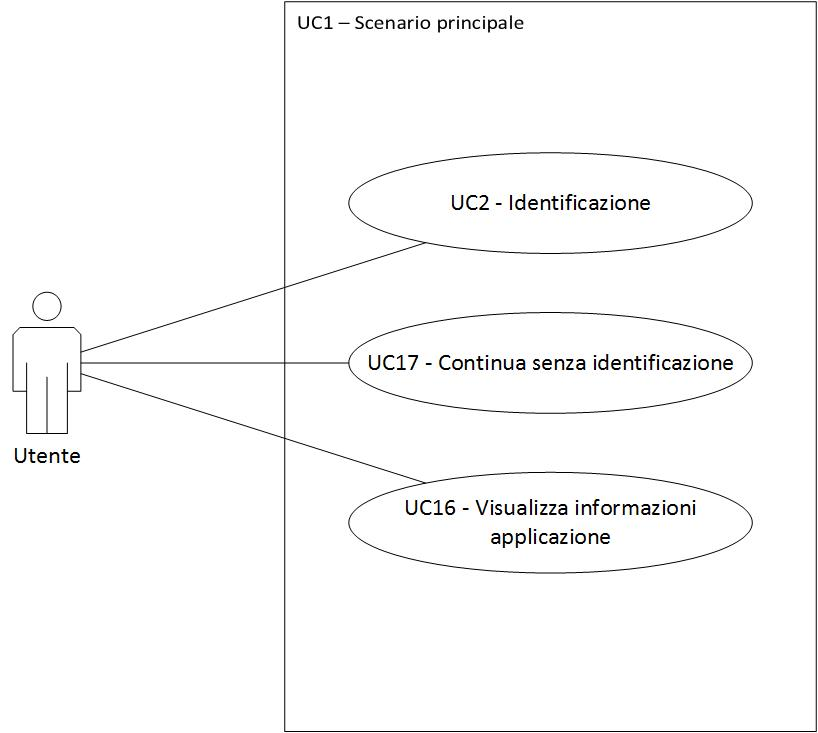
\includegraphics[scale=0.35]{immagini/analisi/UC01_scenario_principale.jpg}
	\caption{\textit{Schema UML Pagina di identificazione}}
\end{figure}\FloatBarrier

\begin{figure}[ht]
	\centering
	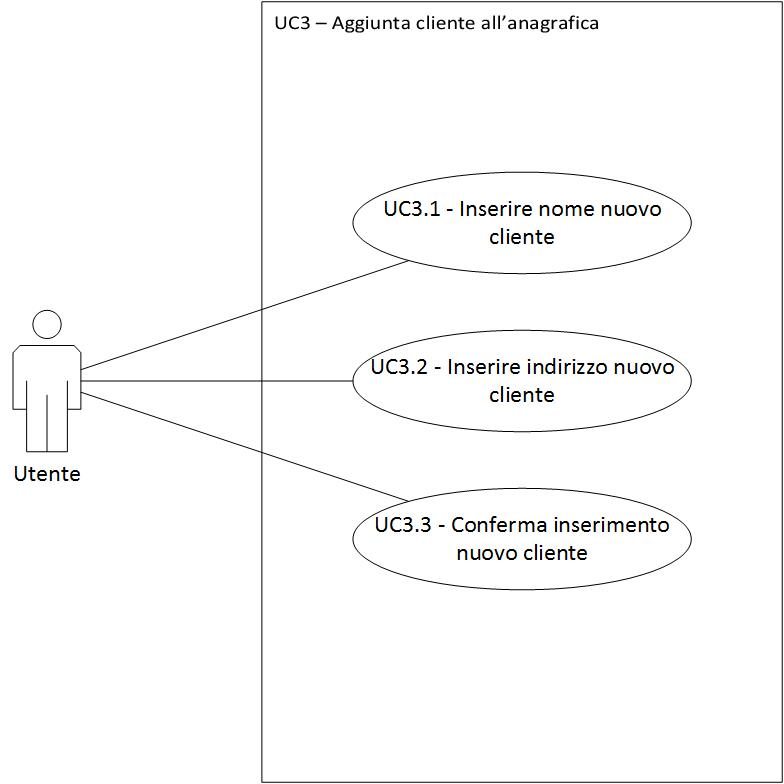
\includegraphics[scale=0.35]{immagini/analisi/UC03_aggiunta_cliente_anagrafica.jpg}
	\caption{\textit{Schema UML Pagina di aggiunta anagrafica cliente}}
\end{figure}\FloatBarrier


\section{Diagrammi di Attività}
Come parte finale dell'analisi dei requisiti ho presentato dei diagrammi di attività per chiarire il flusso di attività intrapreso dall'applicativo in varie schermate: di seguito un esempio di diagramma creato durante l'attività di analisi:

\begin{figure}[ht]
	\centering
	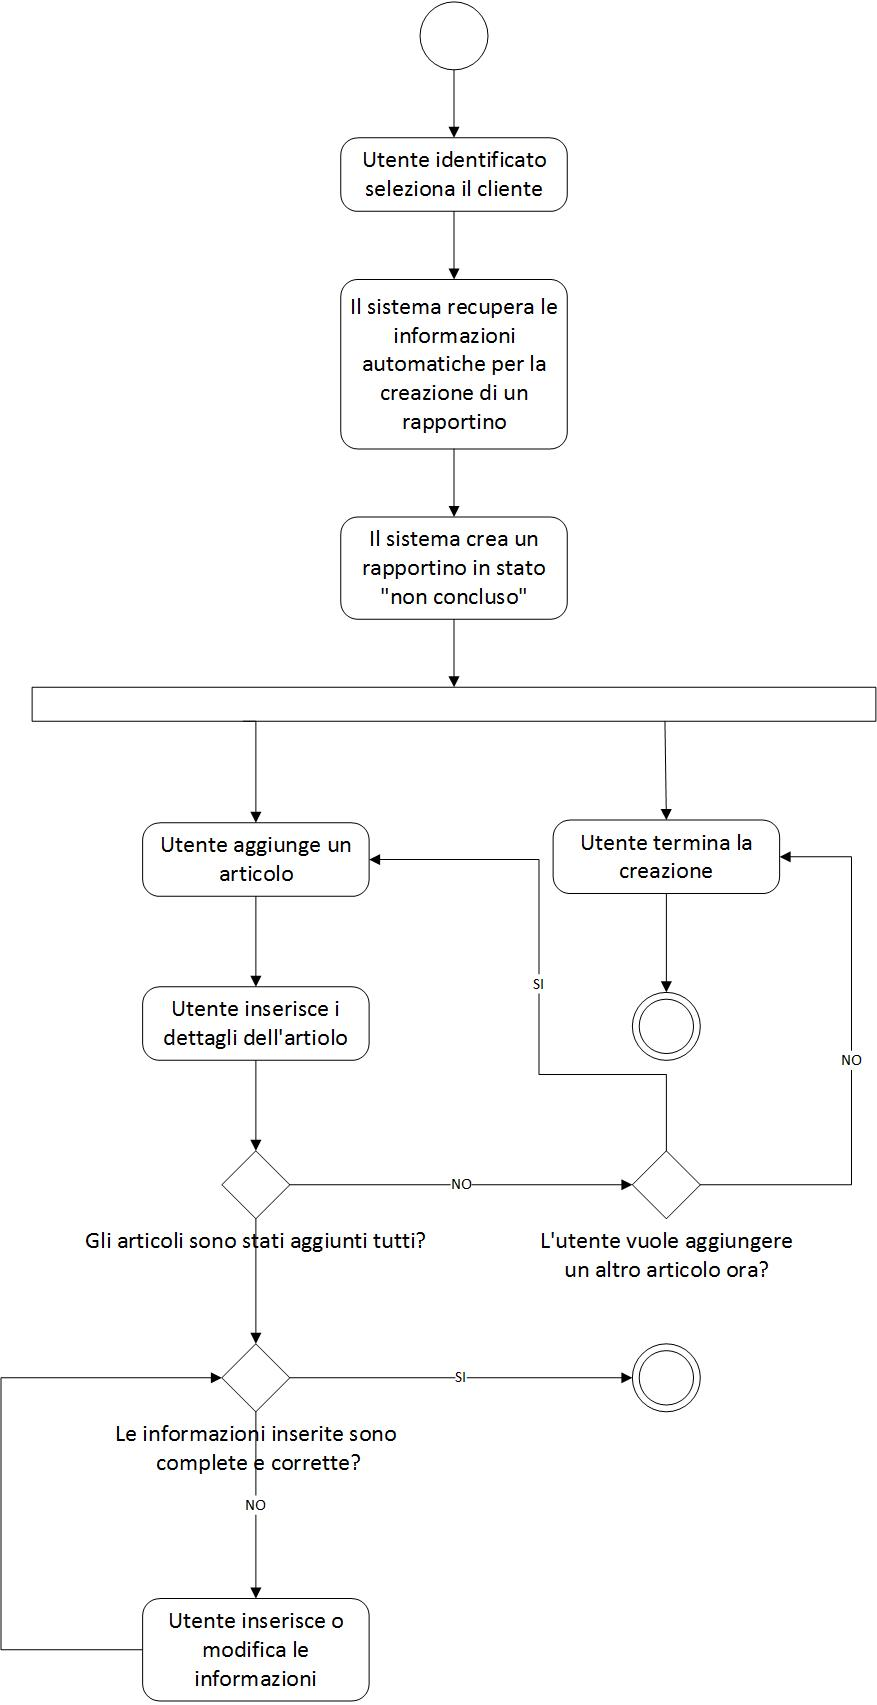
\includegraphics[scale=0.52]{immagini/analisi/003_creazione_rapportino.jpg}
	\caption{\textit{Diagramma Attività di creazione del rapportino}}
\end{figure}\FloatBarrier



             % Analisi
\newpage
%**************************************************************
\chapter{Progettazione e codifica}
\label{cap:progettazione-codifica}
\section{Funzioni di Xamarin.Forms}
Xamarin.Forms è un \textit{framework\ped{G}} rilasciato da Xamarin nel 2014 e successivamente acquistato da \textit{Microsoft\ped{G}}; permette di sviluppare \textit{UI\ped{G}} che possono essere condivise tra i maggiori \textit{sistemi operativi\ped{G}} mobile: \textit{Android\ped{G}. iOS\ped{G}, Windows Phone\ped{G}}. Le interfacce condivise vendono renderizzate usando controlli nativi della piattaforma utilizzata, consentendo ad applicativi Xamarin.Forms di mantenere il \textit{look and feel\ped{G}} appropriato al dispositivo in uso. \\
Le applicazioni Xamarin.Forms sono viste come native dai dispositivi e consentono di usare qualsiasi \textit{API\ped{G}} o proprietà della piattaforma, rendendo possibile la creazione di applicazioni con parte della \textit{UI\ped{G}} strutturata con Xamarin.Forms ed altre create usando strumenti nativi.
\subsection{C\# e XAML}
Per creare le \textit{UI\ped{G}} in Xamarin.Forms sono stati due approcci:
\begin{itemize}
	\item \textbf{Codice C\#}: si utilizzano le ricche \textit{API\ped{G}} provviste da Xamarin.Forms per creare interamente le \textit{UI\ped{G}}
	\item \textbf{XAML}: un linguaggio dichiaritivo di \textit{Markup\ped{G}} di \textit{Microsoft\ped{G}}, che definisce l'\textit{interfaccia\ped{G}} su un file \textit{XML\ped{G}} usando sintassi XAML, mentre il comportamento in runtime è definito da un file separato.
\end{itemize}
Per il progetto è stato scelto l'utilizzo di \textit{XAML\ped{G}}, vista la scelta di utilizzare un \textit{Design Pattern\ped{G}} architetturale \textit{Model View ViewModel\ped{G}}. Infatti, questo \textit{Design Pattern\ped{G}} permette la separazione totale tra modello di dati, comportamento e vista dell'applicazione, e l'uso di un linguaggio di \textit{Markup\ped{G}} lo sposa appieno, permettendo di fatto il \textit{Two-way Data-Binding\ped{G}} che sarà discusso in seguito.
\subsection{Tipologia di condivisione del codice}
Le applicazioni Xamarin.Forms sono strutturate come le applicazioni multi-piattaforma tradizionali, sfruttando l'approccio più comune di usare una \textit{PCL\ped{G}} oppure un \textit{Shared Project\ped{G}} per contenere il codice condiviso e, quindi, creare applicazioni specifiche per ogni piattaforma che sfruttino tale codice. 
\subsubsection{PCL}
Tradizionalmente, creando un'applicazione o una libreria, la \textit{DLL\ped{G}} risultante è limitata a funzionare per la piattaforma per cui è stata sviluppata, impedendo, per esempio, l'utilizzo di un \textit{assembly\ped{G}} per un'applicazione \textit{Android\ped{G}} all'interno di \textit{Windows Phone\ped{G}} o \textit{iOS\ped{G}}.
\\
Nella creazione di una \textit{PCL\ped{G}} è invece possibile definire una combinazione di piattaforme nelle quali si vuole farla funzionare, creando un identificatore di profilo che specifica quali piattaforme sono supportate dalla libreria risultante.

\begin{figure}[ht]
	\centering
	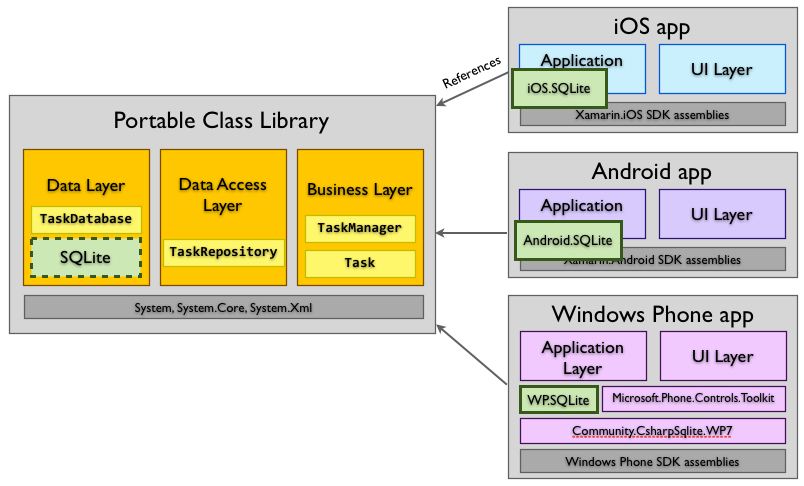
\includegraphics[scale=0.30]{immagini/progettazione/PortableClassLibrary.png}
	\caption{\textit{Architettura Xamarin.Forms PCL}}
\end{figure}\FloatBarrier

Vi sono diversi pro e contro nell'utilizzo delle PCL:
\begin{itemize}
	\item \textbf{PRO:} condivisione del codice centralizzata: il codice scritto e testato all'interno di un progetto singolo può poi essere riutilizzato da altre librerie o applicazioni.
	\item \textbf{PRO:} effettuando il \textit{Refactoring\ped{G}} viene modificato tutto il codice caricato nella soluzione, sia nella \textit{PCL\ped{G}}che nei progetti specifici per piattaforma.
	\item \textbf{PRO:} il progetto \textit{PCL\ped{G}} può essere facilmente referenziato da altri progetti in una soluzione, oppure l'\textit{assembly\ped{G}} risultante può essere condiviso perché altri lo referenzino nelle loro soluzioni.
	\item \textbf{CONTRO} la \textit{PCL\ped{G}} potendo essere condivisa con diverse applicazioni, le librerie specifiche per la piattaforma non possono essere riferite direttamente.
	\item \textbf{CONTRO} la \textit{PCL\ped{G}} non può includere classi fruibili contemporaneamente in \textit{MonoTouch\ped{G}} e \textit{Mono for Android\ped{G}}. 
\end{itemize}
Tuttavia i problemi possono essere parzialmente risolti sfruttando il \textit{Dependency Service\ped{G}} provvisto da Xamarin, che consente di codificare implementazioni specifiche per piattaforma in un' \textit{interfaccia\ped{G}} definita nella \textit{PCL\ped{G}}.
\subsubsection{Shared project}
Contrariamente agli altri approcci, un progetto condiviso non risulta inserito nella creazione di una \textit{DLL\ped{G}}; il codice viene invece compilato in ciascun progetto che lo referenzia, facendo in modo che ogni progetto condiviso referenziato venga compilato come se fosse dello stesso.
\\
Un progetto consiviso può contenere direttiveche ne disabilitano alcune sezioni, secondo la piattaforma su cui viene eseguito il codice.

\begin{figure}[ht]
	\centering
	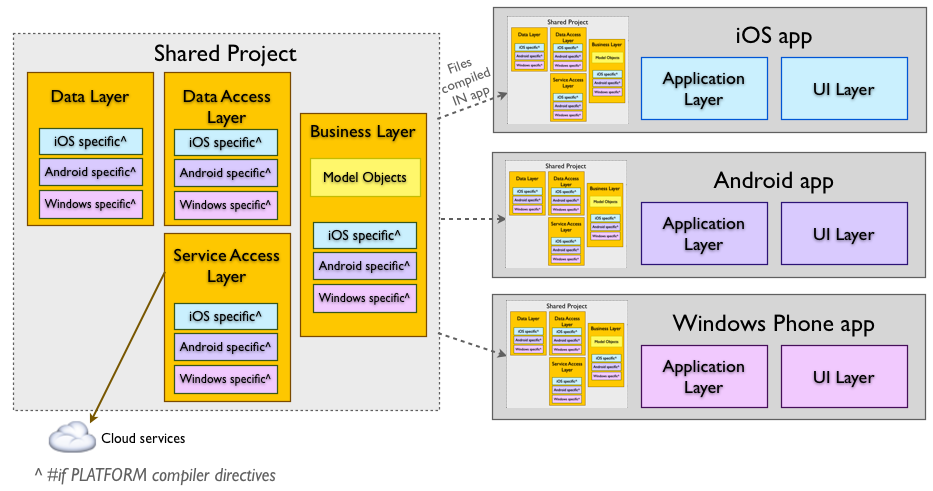
\includegraphics[scale=0.30]{immagini/progettazione/SharedAssetProject.png}
	\caption{\textit{Architettura Xamarin.Forms Shared Project}}
\end{figure}\FloatBarrier

Poichè un progetto condiviso non può essere compilato singolarmente, ma va effettivamente inserito nei progetti che lo referenziano, non può a sua volta referenziare altri progetti, nemmeno altri progetti condivisi.

\subsubsection{Approccio scelto}

Per lo sviluppo dell'applicativo è stato scelto di adottare l'approccio \textit{cross-platform\ped{G}} basato su \textit{PCL\ped{G}}; infatti, considerato che il codice scritto deve essere fruibile da ogni \textit{sistema operativo\ped{G}}, compilare parti specifiche per ogni piattaforma avrebbe complicato l'architettura del progetto. 
\subsection{Progettazione dell'interfaccia grafica}
Xamarin.Forms fornisce una singola \textit{API\ped{G}} per lo sviluppo di \textit{UI\ped{G}}, che traduce a \textit{runtime\ped{G}} i controlli di Xamarin.Forms negli appropriati controlli nativi della piattaforma, per poi renderizzarli.
\\
Per la creazione di \textit{UI\ped{G}}, sono fornite \textbf{quattro classi} principali, che possono essere combinate per realizzare le interfacce desiderate:
\begin{enumerate}
	\item \textbf{Page:} è un elemento visuale che ricopre totalmente, o quasi, lo schermo del dispositivo e contiene una singolo foglio.
	
	\begin{figure}[ht]
		\centering
		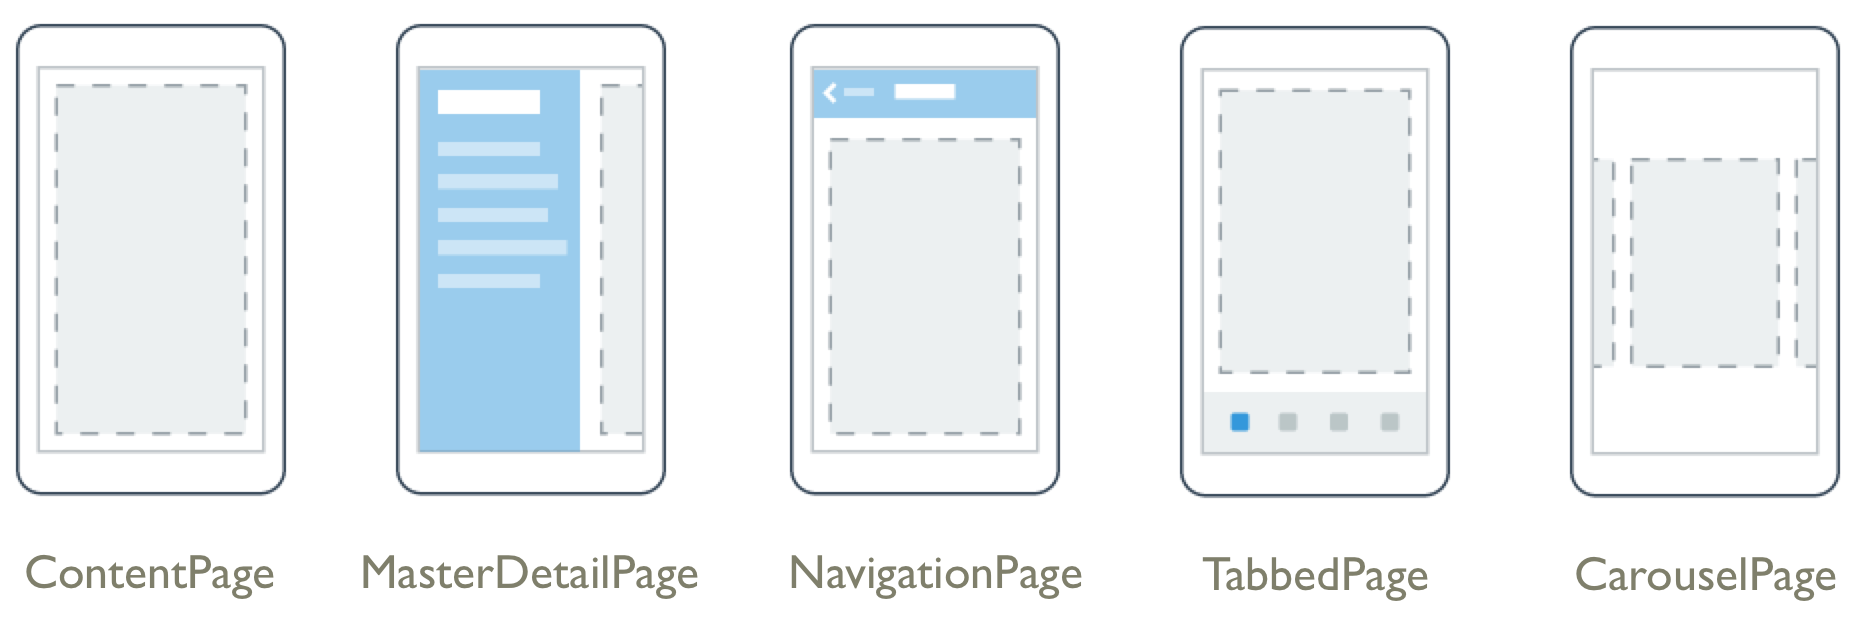
\includegraphics[scale=0.25]{immagini/progettazione/page-types.png}
		\caption{\textit{Tipi di \textbf{Page} fornite da Xamarin.Forms}}
	\end{figure}\FloatBarrier
	
	\item \textbf{Layout:} sono una specializzazione della classe \textbf{View}; fungono da contenitori per altri \textit{Layout\ped{G}} o controlli e vengono utilizzati per gestireil posizionamento e la dimensione dei contenuti.
	
		\begin{figure}[ht]
			\centering
			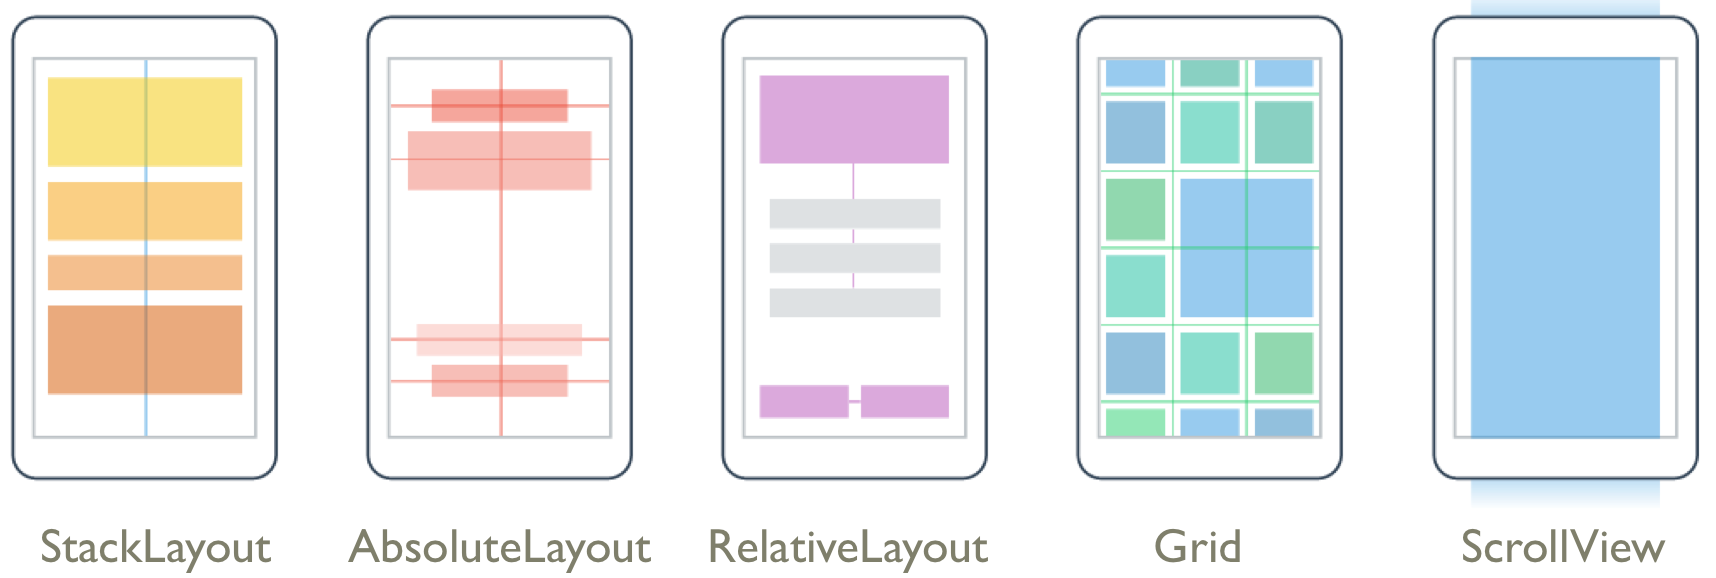
\includegraphics[scale=0.25]{immagini/progettazione/Layouts.png}
			\caption{\textit{Tipi di \textbf{Layout} forniti da Xamarin.Forms}}
		\end{figure}\FloatBarrier
		
		\item \textbf{View:} sono definiti \textit{View\ped{G}} tutti gli elementi grafici, come i pulsanti, le etichette, gli inserimenti di testo. Tutti questi elementi vengono coordinati allo stile grafico tipico della piattaforma usata.
		
		\item \textbf{Cells:} è un elemento usato per realizzare oggetti nelle liste o nelle tabelle e specifica come ogni oggetto nella lista deve essere visualizzato. Una cella dunque non è un elemento grafico, ma una struttura per creare diversi elementi grafici, fornendo le caratteristiche di base di ogni cella
		
\end{enumerate}

\subsection{Data Binding}
Xamarin.Forms usa il \textit{Data-Binding} per semplificare come le interfacce utente delle applicazioni interagiscono con i dati sottostanti. 
\\
Il \textit{Data-Binding\ped{G}} definisce la relazione tra due oggetti, la sorgente provvede i dati mentre il bersaglio li usa, solitamente mostrandoli a video. Nel progetto è stato usato un \textit{framework\ped{G}} per semplificare l'utilizzo di \textit{MVVM\ped{G}} con il \textit{Data-Binding\ped{G}}. \textit{MVVMLight\ped{G}} permette di avere delle strutture già pronte che permettono facilmente di collegare le \textit{Property\ped{G}} dei \textit{ViewModel\ped{G}} con le componenti grafiche per eseguire il \textit{Data-Binding\ped{G}}.

\subsection{Accesso a funzioni native}
Nell'applicativo spesso si deve richiedere delle funzioni specifiche della piattaforma. In un progetto \textit{PCL\ped{G}} non è possibile scrivere codice nativo direttamente nel progetto portabile, si deve dunque utilizzare delle tecniche per richiamare metodi scritti nel codice nativo della piattaforma.
 
\subsubsection{Dependency Service}
Xamarin.Forms fornisce un semplice metodo per implementare funzionalità native delle piattaforme che non sono facilmente condivisibili tra loro, il \textit{Dependency Service\ped{G}}, e il suo funzionamento prevede tre parti:
\begin{itemize}
	\item \textbf{Interfaccia:} una classe interfaccia nel codice condiviso che definisce le funzionalità che richiedono codice specifico per la piattaforma.
	\item \textbf{Registrazione:} un'implementazione dell'interfaccia in ogni progetto dell'applicazione, con allegato un attributo che registri la classe in modo che il \textit{Dependency Service\ped{G}} possa crearne istanze.
	\item \textbf{Locazione:} chiamando il \textit{Dependency Service\ped{G}} nel codice condiviso si ottinene a runtime un'istanza dell'interfaccia definita, consentendo al codice condiviso di accedere alla piattaforma sottostante.
\end{itemize}

\subsection{Design Pattern}
Durante la fase di progettazione, è stato considerato il \textit{design pattern\ped{G}} architetturale \textit{Model-View-ViewModel} per la separazione della grafica dal contenuto e per semplificare la connessione tra le componenti.
\subsubsection{Model-View-ViewModel}
Il \textit{Model-View-ViewModel\ped{G}} è un \textit{design pattern\ped{G}} architetturale creato da \textit{Microsoft\ped{G}} nel 2005, pensato inizialmente per aiutare lo sviluppo di applicativi \textit{WPF\ped{G}} e \textit{Silverlight\ped{G}}, sfruttando le funzioni di \textit{Data-Binding\textit{G}}.
\\
\textit{MVVM\ped{G}} consente, associato a \textit{XAML\ped{G}}, di sviluppare \textit{UI\ped{G}} in modo completamente indipendente dalla logica, collegando i campi da popolare alla struttura sottostante con \textit{Data-Binding\ped{G}}. Questa profonda separazione tra grafica e logica rende indipendente lo sviluppo delle due parti, semplificando la strutturazione della parte grafica degli applicativi.

\paragraph{Model}
Il model è un'implementazione del \textit{domain model\ped{G}} dell'applicazione, il quale include i dati e la loro logica di business e validazione. Questi sono rappresentanti quindi sia da \textit{database\ped{G}} o altri archivi, sia da oggetti di accesso ai dati.
\paragraph{View}
La View rappresenta l'interfaccia grafica con cui l'utente interagisce, limitandosi a presentare i dati richiesti ed i controlli necessari per gestirli. La View in \textit{MVVM\ped{G}} è attivae gestiche comportamenti, eventi e \textit{Data-Binding\ped{G}} che richiedono una conoscenza del Model sottostante, solitamente mappandoli a proprietà o comandi.
\paragraph{ViewModel}
Il ViewModel si frappone tra View e Model, occupandosi delle iterazioni tra i due, facendo in modo che il Model non venga influenzato da come la View gestisce i suoi dati ed impedendo alla View una connessione diretta con il Model. Il ViewModel espone metodi, dati e comandi neccessari alla View, rispondendo ai suoi \textit{input\ped{G}} con chiamate ai metodi del Model, traducendone i risultati in formati fruibili e lanciando eventi perché la View li utilizzi. Se il Model viene modificato, invia eventi al ViewModel perché ne rilevi le modifiche e faccia in modo che la View agisca di conseguenza.

		\begin{figure}[ht]
			\centering
			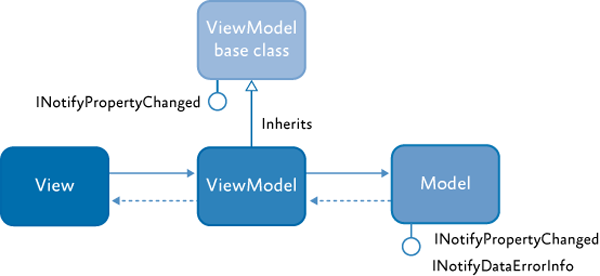
\includegraphics[scale=0.35]{immagini/progettazione/IC448599.png}
			\caption{\textit{Componenti Model-View-ViewModel}}
		\end{figure}\FloatBarrier

\section{Diagramma delle classi}
Al termine della fase di progettazione è stato prodotto uno schema delle classi che è rimasto circoscritto alla libreria condivisa, nel quale è stato cercato di evidenziare l'implementazione del pattern \textit{MVVM\ped{G}}.
\\
Ogni piattaforma contiene un file main, che permette di accedere alla libreria condivisa e creare la \textit{Classe App\ped{G}}, allo scopo di inizializzare l'applicazione.
\\
I componenti dell'applicazione \app sono i componenti imposti dal \textit{design pattern\ped{G}} architetturale \textit{Model-View-ViewModel\ped{G}}
		\begin{figure}[ht]
			\centering
			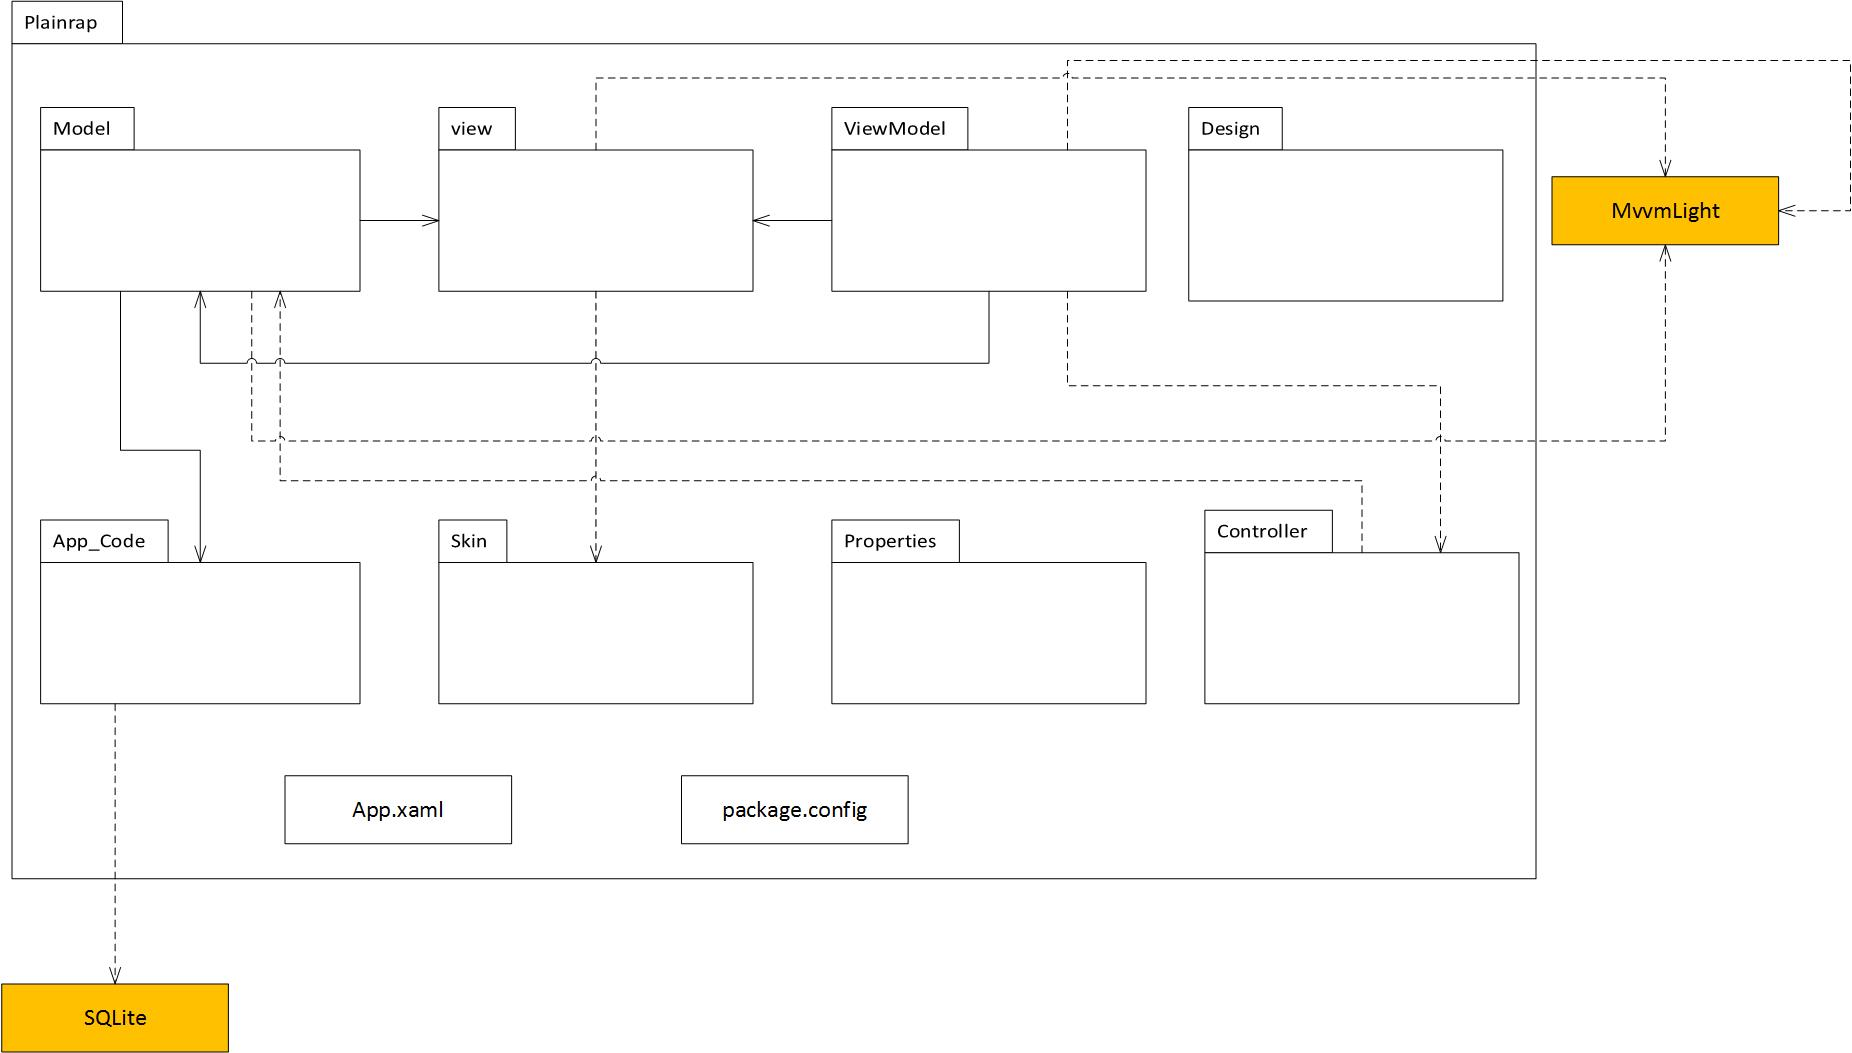
\includegraphics[scale=0.35]{immagini/progettazione/plainrap_portable.jpg}
			\caption{\textit{Componenti Plain.Rap.Mobile}}
		\end{figure}\FloatBarrier
		
		\begin{figure}[ht]
			\centering
			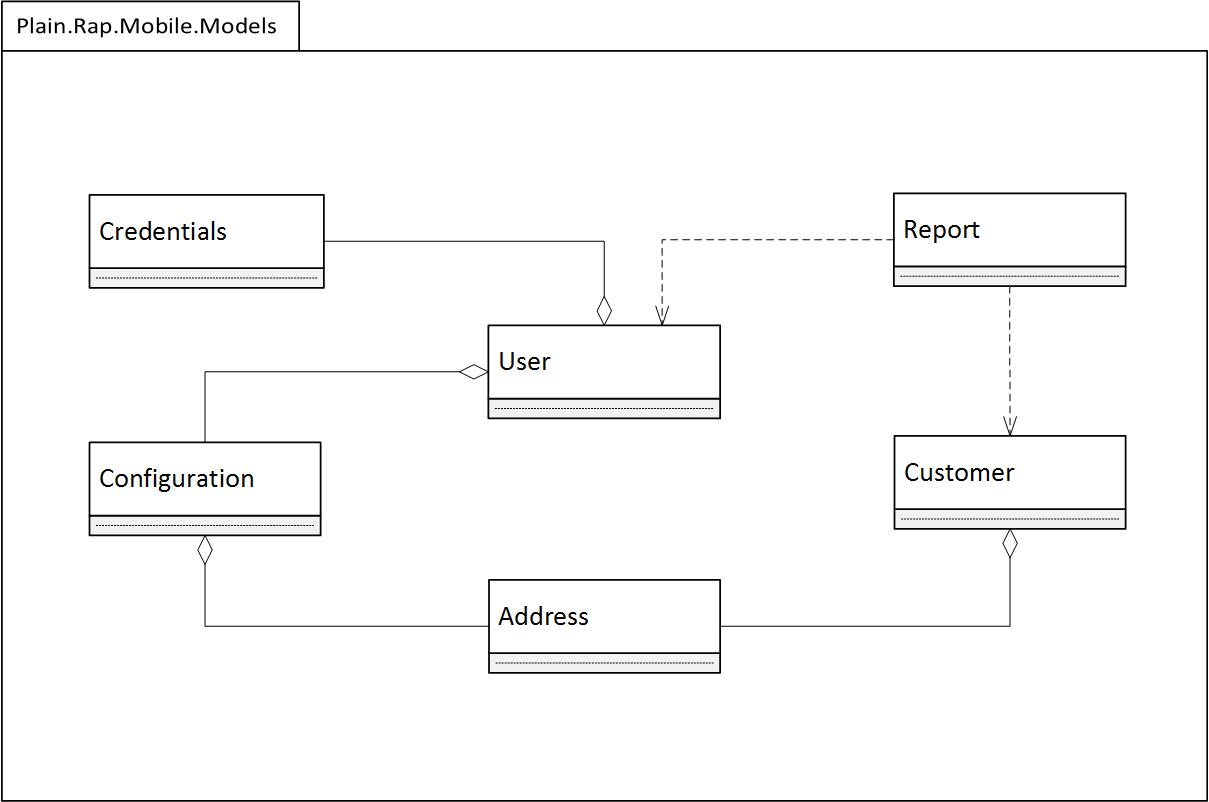
\includegraphics[scale=0.35]{immagini/progettazione/Models.jpg}
			\caption{\textit{Componente Model Plain.Rap.Mobile}}
		\end{figure}\FloatBarrier
		
		\begin{figure}[ht]
			\centering
			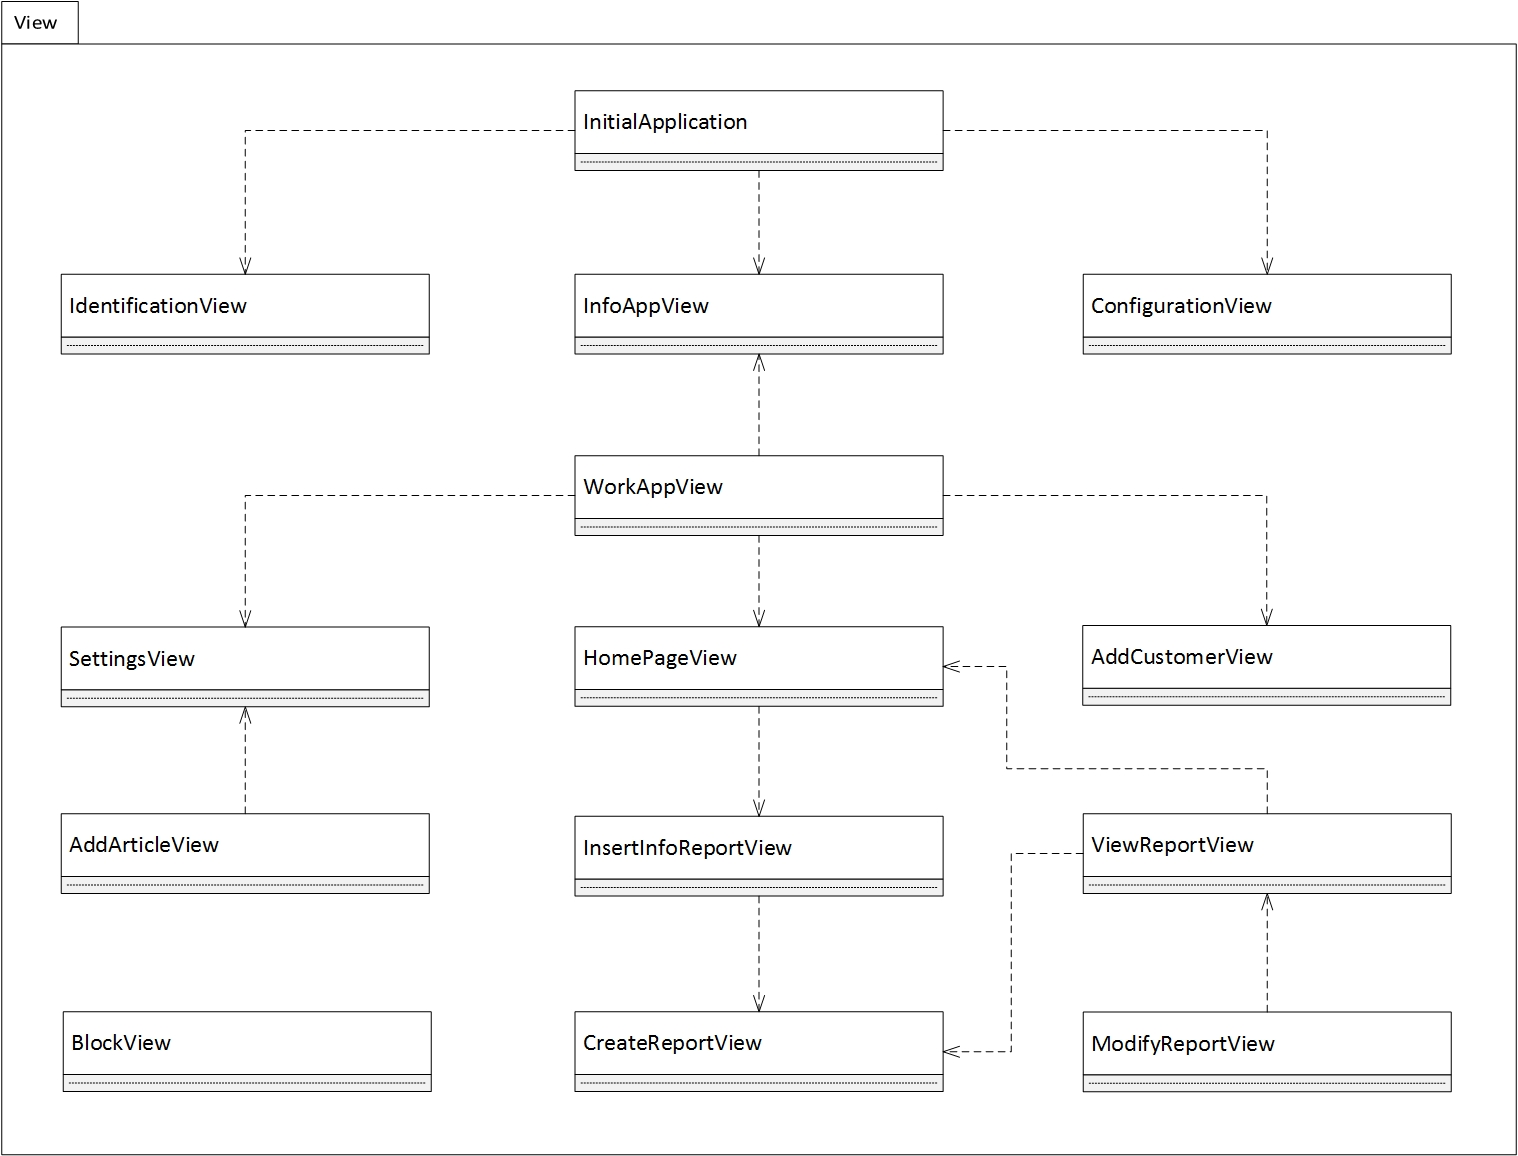
\includegraphics[scale=0.35]{immagini/progettazione/plainrap_view.jpg}
			\caption{\textit{Componente View Plain.Rap.Mobile}}
		\end{figure}\FloatBarrier
		
		\begin{figure}[ht]
			\centering
			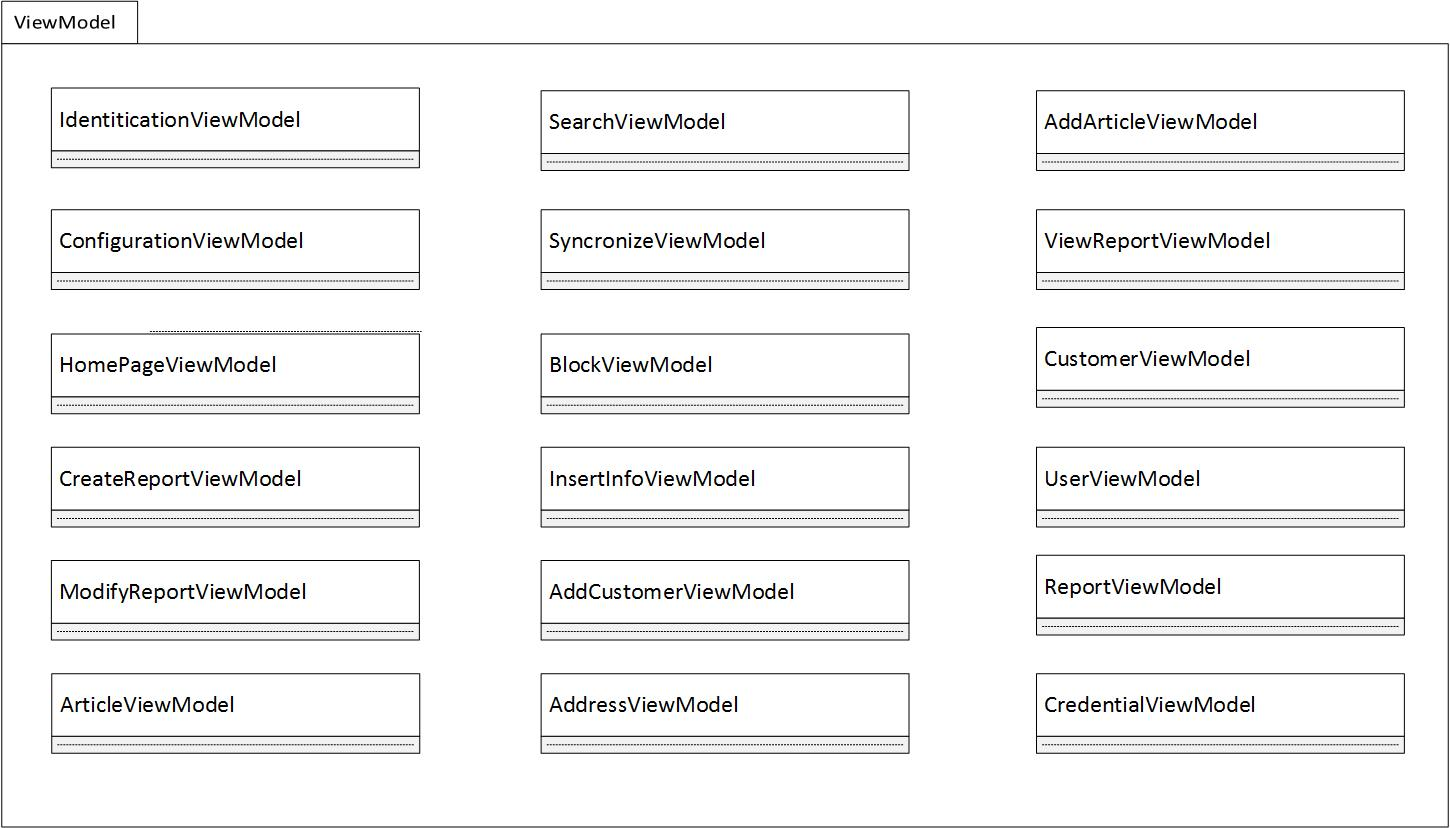
\includegraphics[scale=0.35]{immagini/progettazione/plainrap_viewmodel.jpg}
			\caption{\textit{Componente ViewModel Plain.Rap.Mobile}}
		\end{figure}\FloatBarrier

\section{Strumenti utilizzati}
\subsection{Ambiente di sviluppo}
\subsection{Pacchetti NuGet}
\subsection{SQLite.Net}
\subsection{Newtonsoft.Json}
\subsection{iTextSharp}
\subsection{MVVMLight}
\subsection{Emulator Android for Visual Studio}


             % Progettazione e codifica
\newpage
%**************************************************************
\chapter{Verifica e validazione}
\label{cap:verifica-validazione}				% Funzionalità ottenute
\newpage
\chapter{Conclusioni}
\label{cap:conclusioni}

\section{Test}
Il prototipo dell'applicativo sviluppato durante l'esperienza di stage è stato sottoposto ad una serie di test sia da parte mia, sia dal tutor aziendale, per verificare le funzionalità e la corrispondenza ai requisiti definiti in fase di analisi.
\section{Problematiche riscontrate}
Durante lo sviluppo del'applicativo ho subito numerosi rallentamenti a causa della ricerca della creazione del rapportino a partire da un layout scambiabile. Inizialmente avevo testato le funzionalità fornite da diverse librerie, ma nessuna forniva ciò che realmente interessava all'azienda. L'uso di \textit{XSLT\ped{G}} è stato decretato in ritardo da come stabilito nel piano, questo ha comportato un ritardo sull'inizio dell'analisi, e di conseguenza di tutte le attività successive.  
\section{Esperienza di stage}
Nell'accingermi alla scelta dello stage, ho puntato sopratutto ad un'esperienza che fosse il più possibile paragonabile ad un effettivo impiego lavorativo; contando di essere inserito e trattato, a tutti gli effetti, come un impiegato dell'azienda ospitante, con lo scopo di ottenere una proficua e valida esperienza formativa.
\\
A conclusione dello stage, ritengo che l'esperienza lavorativa compiuta in \asi abbia soddisfatto in pieno le mie aspettative.
\section{Preparazione corso di studi}
Personalmente ritengo che le competenze acquisite durante i tre anni del corso di studi si siano dimostrate adeguate, per un proficuo inserimento nel mondo del lavoro, specializzato nella creazione e commercializzazione di prodotti informatici.

\section{Conoscenze acquisite}
\begin{itemize}
	\item \textbf{Scrum:} durante gli studi universitari non ho mai preso in considerazione di applicare una precisa metodologia per la realizzazione dei vari progetti. Nel corso dello stage, ho potuto invece verificare come Scrum, adottato da \asi, si sia rilevato particolarmente efficiente per gestire le varie fasi di sviluppo del nuovo prodotto. Questa esperienza mi ha permesso di apprendere l'ideologia su cui è basata la creazione di Scrum, ho potuto collaudare il corretto svolgimento di tale metodologia ed ho apprezzato la sua applicazione nei processi aziendali.
	\item \textbf{Sviluppo Mobile:} non avendo mai svolto in precedenza alcun progetto su piattaforme mobili, mi sono sentito particolarmente soddisfatto del risultato ottenuto con lo stage, nel corso del quale ho appreso dettagliatamente come sono gestiti gli applicativi delle varie piattaforme, consentendomi di familiarizzare motlo con lo sviluppo delle applicazioni per dispositivi mobili e di ampliare le mie conoscenze su una disciplina non ancora approfondita nei corsi universitari.
	\item \textbf{Xamarin.Forms:} per sviluppare l'applicativo durante lo stage ho dovuto imparare a conoscere ed utilizzare Xamarin.Forms che si è rilevato uno strumento abbastanza efficace per lo sviluppo \textit{cross-platform\ped{G}}.
\end{itemize}             % Conclusioni  
 \facciatabianca                   
%**************************************************************
% Materiale finale
%**************************************************************
\backmatter
%\printglossaries
% 
\input{glossario}  
\newpage
%**************************************************************
% Bibliografia
%**************************************************************

\cleardoublepage


%\chapter{Bibliografia}

\end{document}